\documentclass[journal,12pt,onecolumn,draftclsnofoot]{article}
%for 
%double spacing
\usepackage{amsmath}
\usepackage{amssymb}
\usepackage{fullpage}
\usepackage[sectionbib]{chapterbib}
\usepackage{subfiles}
\usepackage[noadjust]{cite}
\usepackage[round,numbers]{natbib}
\usepackage{multirow}
\usepackage{booktabs}
\usepackage{graphicx}
\usepackage{float}
\usepackage{../ltx/edcomms}
\usepackage{../ltx/setupComments}
\usepackage{hyperref}
\usepackage{geometry}
\usepackage{changepage}
\usepackage{adjustbox}
\usepackage{graphicx}
\usepackage[section]{placeins} % Prevents floats from floating across sections
\usepackage{tabularx}
\usepackage{ltablex} %% Multi page tables 
\usepackage{amsfonts}
\usepackage{glossaries}
\usepackage{multirow} %% Used for Traceability matrix
\usepackage{listings}
\usepackage{calc}
\usepackage[simplified]{pgf-umlcd}
\usepackage[section]{placeins}
\usepackage{enumitem}
\usepackage{hyperref}
\usepackage{longtable}
\usetikzlibrary{arrows.meta}
\usetikzlibrary{calc}
\usetikzlibrary{positioning}
\usepackage{indentfirst}
\newcolumntype{C}[1]{>{\centering}p{#1}} %% For use with tabularx


% \input{filename.tex}      %will format input document according to base doc, 
%%can nest
% \include{filename.tex} % cant nest
% \subfile{filename.tex} % used to load child docs
% \usepackage{standalone} %used for importing preamble of child docs
% \usepackage[final]{pdfpages.pdf} %used to insert pdf files; final 
%%format[pages=3-6]
%---------------------------
\let\Oldsubsection\subsection
\renewcommand{\subsection}{\FloatBarrier\Oldsubsection}
\let\Oldsubsubsection\subsubsection
\renewcommand{\subsubsection}{\FloatBarrier\Oldsubsubsection}

\newcounter{acnum}
\newcommand{\actheacnum}{AC\theacnum}
\newcommand{\acref}[1]{AC\ref{#1}}

\newcounter{ucnum}
\newcommand{\uctheucnum}{UC\theucnum}
\newcommand{\uref}[1]{UC\ref{#1}}

\newcounter{mnum}
\newcommand{\mthemnum}{M\themnum}
\newcommand{\mref}[1]{M\ref{#1}}
\makeglossary

\setlength\parindent{24pt}
% math things
\newcommand{\ra}{$\rightarrow$}



% 
\definecolor{grey}{RGB}{192,192,192}
\definecolor{applegreen}{rgb}{0.55, 0.71, 0.0}
\lstset{ %
  language=Haskell, morekeywords = {family, kind, pattern, expression},
  literate=
  {+}{{$+$}}1
  {/}{{$/$}}1 
  {*}{{$*$}}1 
  {=}{{$=\,\,\,$}}1
  {==}{{$==$}}1 
  %{/=}{{$\not\equiv$}}2
  {==}{{$\equiv$}}2
  {/=}{{$\not\equiv$}}2
  {>}{{$>$}}1 
  {<}{{$<$}}1 
  {\\}{{$\lambda$}}1
  {\\\\}{{\char`\\\char`\\}}1
  {>>}{$>>$}2 
  {:>>=}{{$:>>=$}}2
  %% {>>=}{{\hspace{6pt}\texttt{$>>=$}\hspace{6pt}}}2
  {->}{{$\rightarrow$} }2 
  {>=}{{$\geq$}}2 {<-}{{$\leftarrow$}}2
  {<=}{{$\leq$}}2 {=>}{{$\Rightarrow$} }2
  {|}{{$\mid$}}1 
  {forall}{{$\forall$}}1
  {exists}{{$\exists$}}1 
  {Nat}{{$\mathbb{N}$}}1
  {:\~:}{{$\equiv$}}2
  {\~}{{$\equiv$}}2
  {`In`}{{$\in$}}1
  {.}{{$\circ$\,\,}}1
  ,
  escapeinside={\%*}{*)},
  deletekeywords={>>,>>=,mapM,mapM_,putStrLn,putStr,toInt,show,and,sequence,String,Bool
    ,True,False,Maybe,id,Show,Ordering,Void,Just,Nothing,Int},
  morekeywords={forall, ::, :},
  postbreak={},
  breaklines=true,                
  breakatwhitespace=true,
  %postbreak={  \mbox{\textcolor{grey}{$\rightarrow$}} },
  breakindent = 0pt,
  breakautoindent = true,
  %moredelim=[is][\itshape]{"}{"},
  morestring=[b]",
  mathescape
}

\newcommand{\hstype}[2][0pt]{\attribute{\hspace*{#1}\lstinline[mathescape]|#2|}}

\newcommand{\hstypectr}[1]{\attribute{\hspace*{10pt}\lstinline[mathescape]|#1|}}

\newcommand{\hsfunc}[2][0pt]{\operation{\hspace*{#1}\lstinline[mathescape]|#2|}}


%\newcommand{\@supervisor}{}
\newcommand{\supervisor}[1]{\renewcommand{\@supervisor}{#1}}


%%\end{filecontents*}
\makeindex

\begin{document}
%\maketitle %% Title page included from Title.tex
\begin{titlepage}
    \begin{center}
        \vspace*{1cm}
        
        \textbf{ Event control action rules for Ampersand}
        
             
        \vspace{1.5cm}
        
        \textbf{Yuriy Toporovskyy (toporoy)\\ Yash Sapra (sapray) \\ Jaeden Guo 
    (guoy34)}
        
        \vfill
        
        Supervised by: Dr. Wolfram Kahl
        
        \vspace{0.8cm}
        
        
\includegraphics[width=0.4\textwidth]{../figures/mac_logo.jpg}
        
        Department of Computing and Software\\
        McMaster University\\
        Ontario, Canada\\
        \today
 
        \vfill 

        The authors herewith license the code which this document accompanies under the GPL v.~3, 
        whose full license text can be found in the source repository. 

    \end{center}
\end{titlepage}

\newpage


\begin{abstract}
%light description
Ampersand Tarski is a tool used to produce functional software documents based 
on business process requirements. At times, logical 
discrepancies arise when system changes occur which violate the 
restrictions set forth by the user. When a system violation occurs, one of two 
things can happen: the change that is meant to take place is adjusted (where it 
no longer violates the rules of the system) or the change is discarded. The 
purpose of Event-Condition-Action rules for Ampersand (EFA) is to replace the 
Ampersand's exec-engine which is used to fix system violations. Although the 
exec-engine appears to fix violations in the prototype, manual labour is 
required to fix system invariants inside of Ampersand. The EFA project was 
\edcomm{JG}{ proposed might not be the right word}
proposed to replace the exec-engine by correctly translating ECA rules and 
implementing them as SQL 
queries so that system violations may be automatically corrected. EFA is 
automated and requires no additional work from the user. In addition, EFA is 
provably correct and has a high degree of modularity as it only relies on 
Ampersand's essential components.
\end{abstract}
\newpage
\tableofcontents
\newpage
\newpage
\section{Introduction}\label{Intro}

This document is a guide for the EFA project and includes an brief 
introduction 
to Ampersand, the software requirements used to implement EFA, a section on 
software development, which describes what each module of EFA contains, and 
lastly, a section on software testing.

\subsection{Document Guide}

This document acts as a comprehensive guide to EFA, the first chapter covers 
the basics of Ampersand, the purpose of the project, the intended audience 
(i.e. our stakeholders), tools used to run Ampersand and terminology which will 
be used throughout this guide. 

The second chapter provides an overview of EFA's requirements specifications; 
it is divided into Ampersand system requirements and the EFA project 
requirements.The third section focuses on design implementation and provides 
key information 
on EFA modules. In addition, it provides an outline of the AMMBR algorithm, 
which is used to generate ECA rules and communication protocols which explains 
how EFA communicates with Ampersand's front end. A lot of the proof written to 
verify EFA's correctness is embedded within each module which is covered in 
this section. 

The fourth section covers testing, specifically, it covers property testing 
using QuickCheck and testing MySQL queries using WorkBench. Lastly, the 
Appendix 
covers a variety of information such as tips for setting up 
Ampersand and notes on issues that came up during the course of EFA's 
implementation. 

\subsection{Ampersand}

\indent
The motivation behind Ampersand comes from requirements engineering, which is a 
large part of designing software systems. One of the greatest challenges of 
requirements engineering is translating informal business requirements into 
formal functional specification. Business requirements contain ambiguity 
because they are written in a natural language with the intention of being 
easily understood by humans; however,
functional specifications must be written in a formal language that is 
unambiguous and precise. Typically, this translation of business requirements 
to a formal specification is done by a requirements
engineer, which can be prone to human error.

Ampersand offers an alternative solution which translates the natural language 
used in business process into requirement specifications \cite{ruledesign}. 
Ampersand is a 
software system which offers many tools that aid their clients in the 
translation process from business requirement to formal requirement 
specifications. EFA is implemented as an internal component of Ampersand that 
is meant to automate the correction of system invariants. EFA helps reduce the 
amount of manual labour required by the user by executing SQL queries to fix 
data violations. %---- edit here 

Given a set of data and a set of rules used to operate on the data, Ampersand 
is able to determine if there are discrepancies between the two sets. 
Discrepancies often occur when changes are made to the set of data Ampersand is 
given or to the set of rules that as associated with them. Data discrepancies 
are violations or illegal transactions that occur in the Ampersand system when 
a set of data fails to follow the rules given by the user. When a system 
violation occurs, one of two things can happen: the change that is meant to 
take place is adjusted (where it no longer violates the rules the user 
provides) or the change is discarded. EFA enhances the Ampersand system by 
translating ECA rules and executing them as SQL queries to correct system 
violations and safeguard the database from wrongful transactions.

\subsubsection{Ampersand In Practice}

The Ampersand system is implemented in Haskell and relies on external software 
tools to help generate a prototype and its supporting documents. On windows, 
there is an executable available, but on Linux and Mac operating systems it 
requires installing stack (The Haskell Tool Stack) to build Ampersand from 
source. 
Instructions on how to install the tools and components listed in this section 
can be found in the appendix.

\subsubsection*{The Haskell Platform}
\noindent
Ampersand's most current version requires 
\href{https://www.haskell.org/platform/}{the Haskell Platform 7.10 }. It is 
used to compile Ampersand source code.


\subsubsection*{Ampersand's GitHub}\label{Github}
\noindent
Github hosts the most current version of the Ampersand system. Github is used 
to maintain consistency between the main Ampersand branch and this project. The 
most recent version of Ampersand can be found at 
\href{https://github.com/AmpersandTarski}{Ampersand Tarski's Github }


\subsubsection*{Graphviz}
\noindent
\href{http://www.softpedia.com/get/Others/Miscellaneous/Graphviz.shtml}{Graphviz}
 is an open source graph visualization software that Ampersand uses to generate 
 artifacts, specifically it is used to create graphics for the prototype's 
 requirement documentation. Graphviz is able to take descriptions of graphs in 
 simple text and create diagrams from them. 

\subsubsection*{The Cabal System}
\noindent
\href{https://www.haskell.org/cabal/}{The Cabal System} is used for building 
and packaging Haskell libraries and programs. 
Cabal describes what a Haskell package is, how these packages interact with the 
language, and what must be implemented to support the packages that are used. 
It is part of a larger infrastructure used to distribute, organize, and catalog 
Haskell programs and their associated libraries. \cite{hackage}

\subsubsection*{The Haskell Tool Stack}
\noindent
\href{https://www.haskell.org/cabal/}{The Haskell Tool Stack} is used to 
install the most recent version of Ampersand from source code, and various 
Haskell packages (e.g., QuickCheck).

\subsubsection*{QuickCheck}
\noindent
\href{https://hackage.haskell.org/package/QuickCheck}{QuickCheck} is used to 
test properties of functions used in EFA's modules. QuickCheck is a library for 
random testing of program properties; a programmer simply provides a 
specification of properties which functions should satisfy and QuickCheck 
generates a large number of random cases to test these properties. QuickCheck 
comes with a
\href{http://www.cse.chalmers.se/~rjmh/QuickCheck/manual.html}{manual} on how 
properties can be defined and used. 

\subsubsection*{MySQL WorkBench}
\noindent
\href{https://dev.mysql.com/doc/workbench/en/}{MySQL WorkBench} is used to test 
the SQL queries generated by EFA. MySQL WorkBench is a graphical tool for MySQL 
databases and comes with a build-in editor, in this project it is used to 
manually test queries. Through various stages in development it is used for 
data modeling.

\subsection{Naming Conventions and Terminology}\label{sec:Naming} 
\begin{description}
    \item[ECA] Stands for Event-Condition Action. The rule structure used for 
    data
    bases and commonly used in market ready business rule engines. ECA rules are
    used in Ampersand to describe how a database should be modified in response 
    to
    a system constraint becoming untrue. 
    
    \item [ADL] Stands for ``Abstract Data Language'' (\cite[13]{derFun}). From 
    a
    given set of formally defined business requirements, Ampersand generates a
    functional specification consisting of a data model, a service catalog, a
    formal specification of the services, and a function point analysis. An ADL
    script acts as an input for Ampersand. An ADL file consists of a plain ASCII
    text file.
    
    \item [Ampersand] Ampersand is the name of this project. It is used to 
    refer to
    both the method of generating functional specification from formalized
    business requirements, and the software tool which implements this method.
    
    \item [Business requirements] Requirements which exist due to some real 
    world 
    constraints (i.e. financial, logistic, physical or safety constraints). 
    
    \item [Business rules] See \emph{Business Requirements}.
    
    \item [EFA] Stands for ``ECA (see above) for Ampersand''. This term is used 
    to 
    refer to the contribution of this project. 
    
    \item [Functional specification] A \emph{formal} document which details the 
    operation,
    capabilities, and appearance of a software system. 
    
    \item [Natural language] Language written in a manner similar to that of 
    human 
    communication; language intended to be interpreted and understood by 
    humans, as 
    opposed to machines. 
    
    \item [Requirements engineering] The process of translating business
    requirements into a functional specification. 
    
    \item [Prototype] Ampersand generates a prototype for the user that 
    provides a 
    front-end interface that connects to a back-end database.
    
\end{description}
%\documentclass[document.tex]{subfiles}
%\begin{document}

%%{\section{The Purpose of the Project}\label{sec:Purpose}}
\section{Purpose of the project}
\edcomm{YS}{Added the ``AMMBR section'' based on comments from Dr. Kahl. He has verified the section, I'll follow up with a proof read and other section of this document}

Ampersand follows a \emph{rule based} design principle. Rules are integral to an organization
and these are based on some principles and guidelines set by the organization.
Ampersand uses an ECA (Event-Condition-Action\edcomm{WK}{IMO,
  either ``Event-Condition-Action'' or ``Event --- Condition --- Action''}) approach to make sure all rules are satisfied. An ideal information infrastructure supports employees and other stakeholders to maintain the rules of the business. To maintain a rule means to prevent or correct all violations that might occur due to any external or internal factor.
 
 A large portion of the Ampersand system is already in place; the primary focus of this project was to
augment Ampersand with increased capabilities for automation. The module ``Automatically Fix Violations'' in Figure ~\ref{fig:EFAproject} represents the EFA project and where it fits in the current version of Ampersand.
Ampersand relies on the AMMBR \citep{Ampersand} algorithm to help fix these data violations. 
The role 
of AMMBR in Ampersand is to generate functions which can restore violations
in the generated prototype for the given information system. In AMMBR, human involvement is only limited 
to representing rules (in the ADL files). Before our current project was started, there was no way of actually
applying the AMMBR-generated ECA rules to rule-violating database states.
There was therefore also no means to test whether AMMBR is producing
appropriate ECA rules.

The current state of Ampersand uses, as a work-around, the so-called
``Exec engine''. This requires the author of the ADL file 
to write PHP code operating on strings in order to tell Ampersand
how violations should be fixed. This required the author of the 
ADL file to know PHP and have knowledge of the internals of Ampersand,
essentially making information hiding impossible in Ampersand itself if one wanted to use
the ExecEngine. 
 
The EFA project, an extension to the Ampersand system, allows 
the user of Ampersand to generate a prototype for their information
system in which invariants are automatically maintained by code 
generated by EFA, which is derived from the specification given by the user.

The ECA rules, which act as an input to EFA, are translated into human-readable
SQL. This can later be viewed in the command line using the
\verb|``--print-eca-info''| flag.  The generated SQL queries allow the
correctness of AMMBR to be checked by running code generated by AMMBR on actual
databases. Therefore, EFA will be an essential tool for testing AMMBR.

\begin{figure}[!htb]
\begin{center}
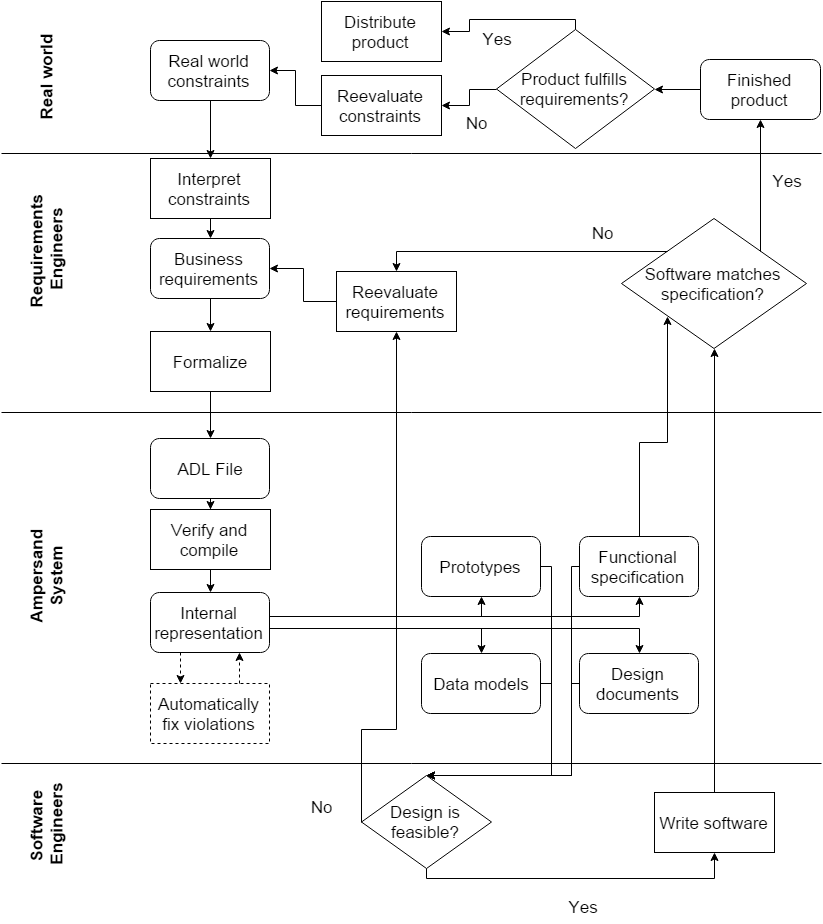
\includegraphics[width=\textwidth]{../figures/business_process}
\caption{Business process diagram representing EFA project represented as a dashed box}~\label{fig:EFAproject}
\end{center}
\end{figure}

\section{The Stakeholders and the intended audience}\label{sec:Stakeholders}
The stake holders of Ampersand are:

\begin{description}
	\item[Ampersand Designers] Responsible for maintaining and developing Ampersand. The overall goal of Ampersand 
is to automate a large part of the software requirements and design process, and EFA fits this goal by greatly increasing
the amount of automation in the system, and therefore decreasing the burden on the user. Furthermore, EFA replaces the ExecEngine,
which allows more of Ampersand to be abstracted and simplifies the maintenance and design of the Ampersand code. 
	\item[The Customer] The requirements engineers using Ampersand to generate prototypes will benefit from the EFA project. 
This will decreases the amount of time 
Ampersand users spend manually inserting PHP code to restore system invariants. The prototypes generated by Ampersand with the 
inclusion of EFA will be less error prone due fewer occurences of violations exposed to the user.
\end{description}

This document is intended to help introduce Ampersand users to EFA 
(ECA rules for Ampersand) -- it provides a basic structure that allows 
individuals to quickly access the information they seek. It is also 
intended to describe the design, implementation, requirements and testing
of EFA for the Ampersand developers. 

\chapter{Functional Requirements}\label{sec:Functional}

This chapter details the functional requirements of EFA, and in particular the
origin of each requirement as well as its priority and relevant test cases.

In the Ampersand system, each transformation which is done on the user
specification of their information system has a reasonable argument of
correctness. While a large part of ensuring this soundness falls to dynamic
testing, many components can be verified by static program analysis, e.g. by the
GHC typechecker and compiler. This requirement for EFA is the same as for
Ampersand - as much information as possible should be modelled by the Haskell
typechecker, which we assume to be sound. Therefore, typechecked programs are
also assumed to be correct with respect to those semantics which have been
encoded on the type level.
 
The Ampersand system also generates a large number and large variety of 
software design and requirements engineering artifacts, including 
documents in various markup formats, graphics and charts, and 
a prototype implementing the business logic encoding in the ADL file.
This large variety of functions must all work independently of 
each other, and in particular not interfere with each others' operation,
which is made very easy by the stateless nature of Haskell. However,
it is still possible to write Haskell code with very complex 
dependencies and code structure, making it very difficult to maintain,
upgrade and debug. EFA is required to be easy to maintain, and therefore
to integrate with the core Ampersand code base easily. 

 The functional requirements of Ampersand can therefore by summarized 
as correctness and modularity. 

\section{System Requirements}
%%-----------------------------SIDE EFFECTS---------------------------------%%
{\setlength{\tabcolsep}{6pt} %% Default is 6
    \begin{tabularx}{\textwidth}{>{\bfseries}m{3cm}X}
        Requirement & S1 \\ 
        \midrule
        \endhead
        Description  & Create pure functions with no unintended side effects
        \\	Rationale & The use of a functional programing languages requires 
        that this program be a pure function and does not have side effects, 
        however certain portions of the code requires the execution of side 
        effects to match the behaviour presented by external programs. In these 
        specific instances, the side effects are an intended behaviour.
        \\	Originator & Stakeholder/Developer
        
        \\ Test Case & Desired results can be confirmed as they will be 
        reflected in changes that take place in the Ampersand database.
        \\	Customer Satisfaction & 5 - Highest 
        \\	Priority & 5 - Highest 
        \vspace{12pt}
    \end{tabularx}
}

%%------------------ MODULES MUST FIT AMPERSAND FRAMEWORK-----------------%%

{\setlength{\tabcolsep}{6pt} %% Default is 6
    \begin{tabularx}{\textwidth}{>{\bfseries}m{3cm}X}
        Requirement & S2 \\ 
        \midrule
        \endhead
        Description  & Added modules must fit within Ampersand's current 
        framework
        \\	Rationale & Ampersand is a huge system that has weekly additions 
        to prevent conflict and breaking of existing packages/modules, an 
        effort should be made to minimize external dependencies. As EFA will be 
        an internal component of Ampersand, if a package that EFA depends on to 
        function properly is no longer maintained and breaks, it will in turn 
        break Ampersand.
        \\	Originator & Ampersand Creators (i.e. our client)        

        \\ Test case & Added modules are tested with cabal build inside of the
        Ampersand system as an internal component (i.e. System testing)
        \\	Customer Satisfaction & 4 - High 
        \\	Priority & 4 - High
        \vspace{12pt}
    \end{tabularx}
}
{\setlength{\tabcolsep}{6pt} %% Default is 6
    \begin{tabularx}{\textwidth}{>{\bfseries}m{3cm}X}
        Requirement & S3 \\ 
        \midrule
        \endhead
        Description  & All code must be maintainable. 
        \\	Rationale & For a system such as Ampersand to be maintainable, all 
        code for each of its components must be well documented so it may be 
        easily understood by those that were not a part of its original 
        development.
        \\	Originator & Ampersand Creators (i.e. our client)        
        
        \\ Test case & A literate program that produces a
        \edchange{WK}{latex}{\LaTeX{}} document. \edcomm{WK}{I do hope
          you still strive to pass this by adding the literate
          documents to the appendix!}
        \\	Customer Satisfaction & 4 - High 
        \\	Priority & 4 - High
        \vspace{12pt}
    \end{tabularx}
}

\section{Project Requirements}
%%--------------------------CORRECTNESS OF ECA TO SQL RULES ------------------%%
{\setlength{\tabcolsep}{6pt} %% Default is 6
    \begin{tabularx}{\textwidth}{>{\bfseries}C{3cm}X}
        Requirement & P1 \\ 
        \midrule
        \endhead
        Description  & Generated SQL queries must preserve the semantics of ECA 
        rules.  
        \\	Rationale & The translation would otherwise not be correct, as the 
        rules would be meaningless if their semantics are lost.
        \\	Originator & Ampersand Creators
        \\ Test Cases & Internal structure of ECA rules can be compared to SQL 
        queries through a series of datatype tests, each of which will result 
        in a traceable result or error message
        \\	Priority & 4 - High
        \vspace{12pt}
    \end{tabularx}
}

%%-------------------------TYPE CORRECTNESS ----------------------------------%%
{\setlength{\tabcolsep}{6pt} %% Default is 6
    \begin{tabularx}{\textwidth}{>{\bfseries}C{3cm}X}
        Requirement & P2 \\ 
        \midrule
        \endhead
        Description  & Provable Correctness: \edcomm{WK}{The use of
          dependent types in TypedSQL establishes some (safety)
          properties, but not the correctness proofs for the
          ECA-to-SQL conversion (see P1) that the Ampersand developers would be
          interested in. In its current form, this ``requirement''
          therefore looks quite confusing/confused.} Haskell like other functional 
        programming languages have 
        a strong type system which can be used for machine-checked proofs.
        \\	Rationale & Curry-Howard correspondence which states that the 
        return type of the function is analogous to a logical theorem, that is 
        subject to the hypothesis corresponding to the types of the argument 
        values that are passed to the function and thus the program used to 
        compute that function is analogous to a proof of that theorem.
        \\	Originator & Ampersand Creators
        \\ Test Cases & Using QuickCheck to test function properties.
        \\	Priority & 4 - High
        \vspace{12pt}
    \end{tabularx}
}

%\edcomm{YS}{Delete : Based on comment from WK, the requirement have been deleted}
%{\setlength{\tabcolsep}{6pt} %% Default is 6
%    \begin{tabularx}{\textwidth}{>{\bfseries}C{3cm}X}
%        Requirement & P3 \\ 
%        \midrule
%        \endhead
%        Description  & Generated SQL queries must be correctly implemented.
%        \edcomm{WK}{What do you mean by this? Would perhaps the
%          syntax- and type-correctness of the SQL statements coming
%          out of TypedSQL, and therewith the rationale of P1, be
%          appropriate here?}
%        \\	Rationale & Ampersand uses a MySQL database, for queries to be 
%        recognized and executed they must be error free. 
%        \\	Originator & Ampersand Creators
%        \\ Test Cases & Using MySQL WorkBench queries are manually executed and 
%        checked for errors.
%        \\	Priority & 4 - High
%        \vspace{12pt}
%    \end{tabularx}
%}


%%%%%%%%%%%%%%%%%%%%%%
%%% Non - Functional Requirements %%%%
%%%%%%%%%%%%%%%%%%%%%%

\chapter{Non-functional Requirements}\label{ch:NonFunc}

%\begin{figure}[!htb]
%	\centering
%	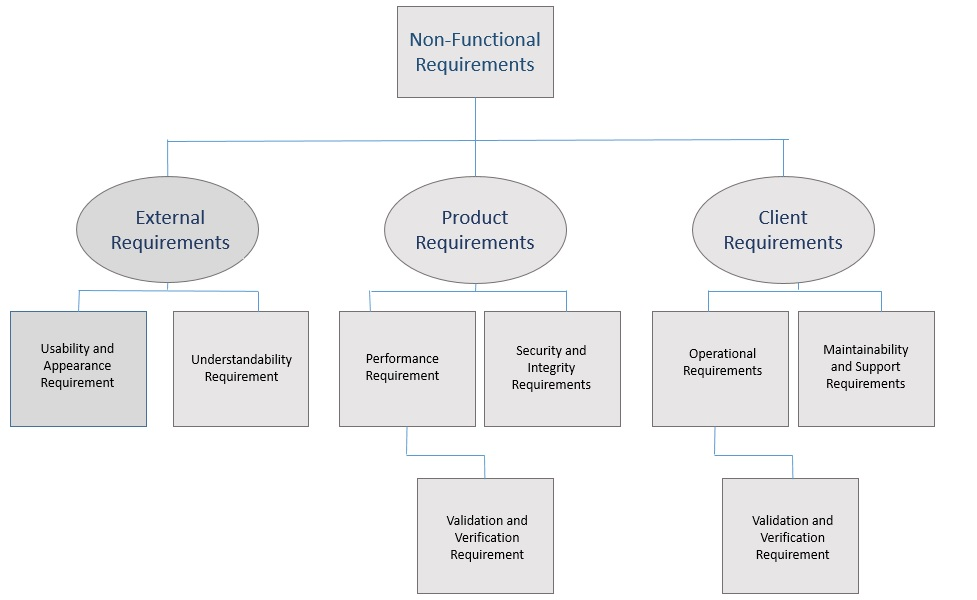
\includegraphics[width=0.8\textwidth]{../figures/NONFUNCTIONAL}
%	\caption{Tree of non-functional requirements as it relates to EFA}~\label{fig:figure2}
%\end{figure}

This chapter briefly describes the various non-functional requirements associated with the EFA project. 

\section{Look and Feel Requirements}\label{sec:LookAndFeel}
\begin{itemize}
    \item The product shall comply with Ampersand standards
    \item The product shall appear readable for Ampersand contributors
\end{itemize}

\section{Usability and Humanity Requirements}\label{sec:Usability}

\begin{itemize}
    \item \textit{Efficiency of use} 
        \begin{itemize}
           \item EFA is easy to use for any Ampersand user.
           \item The user can use EFA with accuracy, as they are provided with 
           the option to use EFA's automated service through the users 
           interface.
        \end{itemize}
    \item \textit{Ease of remembering}  
        \begin{itemize}
            \item EFA does not require the user to memorize protocols
        \end{itemize}
    \item \textit{Error rates} 
        \begin{itemize}
            \item EFA eliminates ECA rule violations caused by the user, 
            EFA's implementation is provably correct through Haskell 
            type-checking system.
        \end{itemize}
       
    \item \textit{Feedback} 
        \begin{itemize}
            \item User receive feed-back concerning the ECA rule 
            violations that have been resolved.
        \end{itemize}
    \item \textit{Overall satisfaction in using the product} 
    \begin{itemize}
        \item Users can be confident in using EFA as it is well tested and 
        provides accurate results which the user can confirm.
    \end{itemize}
\end{itemize}

\subsection{Personalization and Internationalization 
Requirements}\label{subsec:Personalization}
EFA is available only in English but can be adapted for other languages in 
later development versions.

\subsection{Learning Requirements}\label{subsec:LearningReq}
EFA has a shallow learning curve, more time is spent learning the Ampersand 
system. No training is necessary to use EFA as long as the user can operate 
Ampersand.

\section{Understandability and Politeness 
Requirements}\label{sec:Understandability}
Conceptually EFA is easy to understand and users will intuitively know what 
this product does for them. To further understandability, EFA feed back uses 
natural language that is familiar to the user and easy to understand. In 
addition, EFA hides all details of its construction from the user and provides 
the user. 

\ds{What are your understandability requirements for this project?}
\edcomm{JG}{kind of addressed}
\subsection{Accessibility Requirements}\label{Accessibility}
EFA is unable to individually confirm to disability requirements as it is an 
internal component of Ampersand.

\section{Performance Requirements}\label{sec:Performance}
\subsection{Speed and latency Requirements}\label{subsec:SpeedReq}
The use of EFA should not result in a noticeable time delay. EFA shall 
not take more than 3 seconds to complete in the worst case scenario.

\subsection{Safety-Critical Requirements}\label{subec:SafetyReq}
EFA will not expose sensitive information in the Ampersand system to outside 
sources or create new vulnerabilities.

\subsection{Precision or Accuracy Requirements}\label{subsec:AccuracyReq}
SQL queries generated by EFA is correct 100\% of the time with full coverage of 
all ECA rules that apply.
\edcomm{JG}{There's more to be added here, cant think of any right now}
 
\subsection{Reliability and Availability Requirements}\label{subsec:AvailReq}
EFA is available for use anytime Ampersand is used. In the event that Ampersand 
fails, then EFA will also be unavailable as it depends on Ampersand generated 
data taken from the user.

\subsection{Robustness or Fault-Tolerance Requirements}\label{subsec:FaultReq}

In the absence of ECA rule violations, EFA will continue to function and be on 
stand-by until a rule violation is triggered.

\subsection{Capacity Requirements}\label{subsec:CapacityReq}
Ampersand runs on individual machines; EFA as an internal component of 
Ampersand will be able to deal with any amount of data that Ampersand can 
handle. 

\subsection{Scalability and Extensibility 
Requirements}\label{subsec:ScalabilityReq}
EFA is capable of handling large volumes of data, and the translation of ECA 
rules to SQL queries requires a standard amount of time. The number of ECA 
rules is expected to expand as Ampersand etches closer to completion. 

%\subsection{Longevity Requirements}\label{subsec:LongevityReq}
%
%\edcomm{YS}{ECA rules can have interdependencies, these might be buried deep into the rules. Following a certain course of action under EFA, can trigger a deadlock situation where in the system is not able to come up with the best way to deal with inconsistencies in data. In the above example lets say the system is required to give a 2$ discount to the customer if the total cost(including) of his basket is greater than or equal to $10 and provide free shipping, but if the total cost (after discount ) is less than 10$ then 2$ needs to be added for shipping. This creates an infinite loop where the initial cost of the chair is a discount to $8 but then shipping is applied, and it becomes $10, which is again subjected to the discount. EFA needs to take care of such performance issue that would lead the system into a state if deadlock. EFA must have a run time capability to interrupt and send a message to the user about the existence of such conflicting requirements.
%}
%\edcomm{JG}{feel free to add that}
%%	I'm not too sure if the example is valid in our case, Does Ampersand automatically detect such conflicting requirements at an
%%	early stage? I've belive the existence of relational algebra can detect such conflicts, but what if they are introduced at run
%%	later, while the information system is in production?

%% Can you guys come up with a better example? The ones we've listed before don't really capture the performance of EFA

\section{Operational and Environmental Requirements}\label{sec:Operational}
\paragraph*{}
Any system that is currently running Ampersand will be able to run this product 
under a new verion and thus no new requirements have been introduced.
\ds{Either explicitly state the current requirements for running Ampersand, or
mention that any system currently running Ampersand will be able to run
the new version and thus no new requirements have been introduced}.

\section{Maintainability and Support Requirements}\label{sec:Support}
\paragraph*{}
All code submitted for this project must be maintainable, which mean it is well 
documented and comes with mathematical proof. EFA must make sure that each 
specification/error is traceable.
  
\ds{Pull out the explicit requirements and remove the fluff.}

\section{Security and Integrity Requirements}\label{sec:Security}
\paragraph*{}
 Access to the database and software which 
supports the various functions of Ampersand are run locally and subjected to the security system 
the user has in place on his or her work station.

\ds{The git repository is not the issue here, are there any security/integrity
	concerns for the data you will be handling or for the way your contribution
	will handle data?}
\ys{Removed information about git}
	
\section{Validation and Verification Requirements}\label{sec:Verification}
\paragraph*{}
\edcomm{YS}{Section needs to be re-written}

\section{Legal Requirements}\label{sec:Legal}
The implementation must eventually be included in Ampersand, which is licensed
under GPL3. To comply with this license, all of the implementation code must be
either written by us so we may license it under GPL, or must already be licensed
under GPL, or a compatible license, by its original author. We do not plan to
use existing code, other than as a reference.



%%%%%%%%%%%%%%%%%
% Inlcudes sections about 		%
% 1) Purpose of the Project		%
% 2) The stake holder	s 		%
% 	and the intended audience	%
% 3) Implementation Environment %
%%%%%%%%%%%%%%%%%
%%%\documentclass[document.tex]{subfiles}
%\begin{document}

%%{\section{The Purpose of the Project}\label{sec:Purpose}}
\section{Purpose of the project}
\edcomm{YS}{Added the ``AMMBR section'' based on comments from Dr. Kahl. He has verified the section, I'll follow up with a proof read and other section of this document}

Ampersand follows a \emph{rule based} design principle. Rules are integral to an organization
and these are based on some principles and guidelines set by the organization.
Ampersand uses an ECA (Event-Condition-Action\edcomm{WK}{IMO,
  either ``Event-Condition-Action'' or ``Event --- Condition --- Action''}) approach to make sure all rules are satisfied. An ideal information infrastructure supports employees and other stakeholders to maintain the rules of the business. To maintain a rule means to prevent or correct all violations that might occur due to any external or internal factor.
 
 A large portion of the Ampersand system is already in place; the primary focus of this project was to
augment Ampersand with increased capabilities for automation. The module ``Automatically Fix Violations'' in Figure ~\ref{fig:EFAproject} represents the EFA project and where it fits in the current version of Ampersand.
Ampersand relies on the AMMBR \citep{Ampersand} algorithm to help fix these data violations. 
The role 
of AMMBR in Ampersand is to generate functions which can restore violations
in the generated prototype for the given information system. In AMMBR, human involvement is only limited 
to representing rules (in the ADL files). Before our current project was started, there was no way of actually
applying the AMMBR-generated ECA rules to rule-violating database states.
There was therefore also no means to test whether AMMBR is producing
appropriate ECA rules.

The current state of Ampersand uses, as a work-around, the so-called
``Exec engine''. This requires the author of the ADL file 
to write PHP code operating on strings in order to tell Ampersand
how violations should be fixed. This required the author of the 
ADL file to know PHP and have knowledge of the internals of Ampersand,
essentially making information hiding impossible in Ampersand itself if one wanted to use
the ExecEngine. 
 
The EFA project, an extension to the Ampersand system, allows 
the user of Ampersand to generate a prototype for their information
system in which invariants are automatically maintained by code 
generated by EFA, which is derived from the specification given by the user.

The ECA rules, which act as an input to EFA, are translated into human-readable
SQL. This can later be viewed in the command line using the
\verb|``--print-eca-info''| flag.  The generated SQL queries allow the
correctness of AMMBR to be checked by running code generated by AMMBR on actual
databases. Therefore, EFA will be an essential tool for testing AMMBR.

\begin{figure}[!htb]
\begin{center}
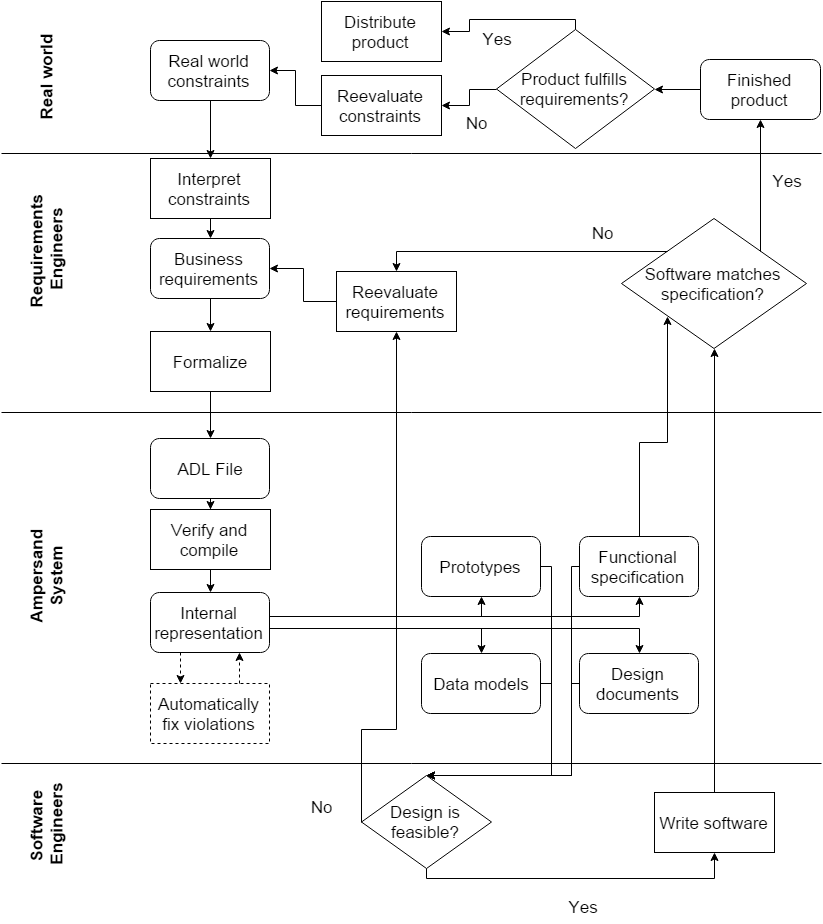
\includegraphics[width=\textwidth]{../figures/business_process}
\caption{Business process diagram representing EFA project represented as a dashed box}~\label{fig:EFAproject}
\end{center}
\end{figure}

\section{The Stakeholders and the intended audience}\label{sec:Stakeholders}
The stake holders of Ampersand are:

\begin{description}
	\item[Ampersand Designers] Responsible for maintaining and developing Ampersand. The overall goal of Ampersand 
is to automate a large part of the software requirements and design process, and EFA fits this goal by greatly increasing
the amount of automation in the system, and therefore decreasing the burden on the user. Furthermore, EFA replaces the ExecEngine,
which allows more of Ampersand to be abstracted and simplifies the maintenance and design of the Ampersand code. 
	\item[The Customer] The requirements engineers using Ampersand to generate prototypes will benefit from the EFA project. 
This will decreases the amount of time 
Ampersand users spend manually inserting PHP code to restore system invariants. The prototypes generated by Ampersand with the 
inclusion of EFA will be less error prone due fewer occurences of violations exposed to the user.
\end{description}

This document is intended to help introduce Ampersand users to EFA 
(ECA rules for Ampersand) -- it provides a basic structure that allows 
individuals to quickly access the information they seek. It is also 
intended to describe the design, implementation, requirements and testing
of EFA for the Ampersand developers. 



%\documentclass[document.tex]{subfiles}
\noindent
\chapter{System Architecture and Module Hierarchy}

This section provides an overview of system architecture and module hierarchy. 
The 
initial section introduces term and tools used in the making of each EFA 
module. The module design is detailed with UML-like class diagrams. However, 
UML class diagrams are typically
used to describe the module systems of object-oriented programs, as opposed to
functional programs. Many of the components of the traditional UML class
diagram are inapplicable to functional programs; therefore, we detail our
modifications to the UML class diagram syntax in 
section ~\ref{subsec:ModuleSyntax}.

Furthermore, the syntax used to describe types and data declarations is not
actual Haskell syntax. The syntax shares many similarities, but several changes
to the syntax are made in this document in order to present the module hierarchy
in a clear manner. These changes are also detailed, in 
section ~\ref{subsec:HaskellSyntax}.

\section{External Libraries}
\noindent No additional dependencies are required outside of those that Ampersand 
already uses. EFA directly uses the following dependencies of Ampersand:
\begin{description}
    \item[Ampersand Core Libraries]
    The EFA project depends on the Ampersand software for the definition of 
    core Data Structures, (\edchange{WK}{i.e.}{i.e.,}\edcomm{WK}{always!} FSpec, which contains the definition of 
    the underlying ECA rules). EFA also maintains the relational schema of 
    the input, and hence, imports Ampersand's existing functions to fetch 
    the table declarations while generating SQL Statements for the ECA 
    rules. AMMBR \cite{AMMBR}, which is the key algorithm responsible for 
    translating business requirements into ECA rules is an integral part of 
    Ampersand.
    \item[simple-sql-parser]
    EFA's pretty printer depends directly on this library for formatting 
    and printing SQL statements. The SQL statement syntax 
    defined here is built on top of the existing expression syntax defined 
    in this package. This package is the one used by the core Ampersand system,
    so our use of it facilitates interaction and integration with Ampersand. 
    \cite{simple-sql}
    \item[wl-pprint] 
    The wl-pprint library\cite{wl-pprint} is a pretty printer based on the
    pretty printing combinators. EFA uses this library in combination with
    the simple-sql-pretty to output the SQL statements in a human readable
    format.
    \item[deepseq]
    The deepseq library provides a type class which implements a function
    for reducing values to normal formal, similarly to the built in
    \lstinline{seq} function.
\end{description}

\noindent
\section{A Description of Haskell-Like Syntax}\label{subsec:HaskellSyntax}

This section details the syntax used to describe the module system of
Ampersand. This syntax largely borrows from actual Haskell syntax, and from the
Agda programming language~\cite{agda}.
Agda is a dependently typed functional
language, and since a large part of our work deals with ``faking'' dependent
types, the syntax of Agda is conducive to easy communication of our module 
system. The
principle of faking dependent types in Haskell is detailed in
Hasochism \citep{hasochism} 
(a portmanteau of Haskell and masochism, because
purportedly wanting to fake dependent types in Haskell is masochism). While the
implementation has since been refined many times over, the general approach is 
still the
same, and will not be detailed here.
While the changes made to the Haskell syntax are reasonably complex, the 
ensuing 
module description becomes vastly simplified. This section is meant to be used
as a reference \edchange{WK}{-}{---} in many cases, the meaning of a type is self-evident. 

\noindent
\subsection*{Description of Types and Kinds}

In the way that a type classifies a set of values, a kind classifies a set of
types. Haskell permits one to define algebraic data types, which are then 
``promoted''
to the kind level \citep{promotion}. 
This permits the type constructor of the datatype to be used
as a kind constructor, and for the value constructors to be used as type 
constructors. In every case in our system, when we define a datatype and use 
the promoted version, we never use the \emph{unpromoted} version. That is, we 
define types which are never used as types, only as kinds, and constructors 
which are never used as value constructors, only type constructors. We write 
\,\,\,
\lstinline!X : A -> B -> $\ldots$ -> Type!
\,\,\, 
to denote a regular data type, and 
\,\,\,
\lstinline!Y : A -> B -> $\ldots$ -> Kind!
\,\,\, 
to denote a datatype
which is used exclusively as a kind. 

\noindent
\subsection*{Description of Dependent types}

The syntax used to denote a ``fake'' dependent type in our model is the same 
as used to denote a real dependent type in Agda. \lstinline!(x : A) -> B! is 
the function
from $x$ to some value of type $B$, where $B$ can mention $x$. This nearly 
looks like a 
real Haskell type --- in Haskell, the syntax would be \texttt{forall (x :: A) . 
B}. However, 
the semantics of these two types are vastly different - the former can pattern 
match
on the value of $x$, while the latter cannot. 

In certain cases, it may be elucidating to see the \emph{real} Haskell type of
an entity (function, datatype, etc.). To differentiate the two, they are typeset
differently, as in this example.

The real type of a function whose type is given as \lstinline!(x : A) -> B! in
our model is \texttt{forall (x :: A) . SingT x -> B}. The type constructor 
\texttt{SingT :: A -> Type}
denotes the singleton type for the kind $A$, which is inhabited by precisely
one value for each type which inhabits $A$. The role and use of singleton types
is detailed further on, in section~\ref{subsec:Singletons}. 

The syntax \lstinline!forall (x : A) -> B! is used to denote the regular
Haskell type \texttt{forall (x :: A) . B}. As is customary in Haskell, the 
quantification
may be dropped when the kind $A$ is clear from the context: 
\lstinline!forall (x : A) -> P x! 
and
\lstinline!forall x -> P x! denote the type \texttt{forall (x :: A) . P x}.

\subsection*{Constraints}

The Haskell syntax \texttt{A -> B} denotes a function from $A$ to $B$. However,
we use the arrow to additionally denote constraints. For example, the function
\texttt{Show a => a -> String} would be written simply as 
\lstinline!Show a -> a -> String!
.
In certain cases, a constraint is intended to be used only in an implicit 
fashion 
(i.e. as an actual constraint), in which case the constraint is written with 
the typical \lstinline{=>} syntax. 

\subsection*{Existential quantification}

The type \lstinline!exists (x : A) (P x)! indicates that there exists some $x$
of kind $A$ which satisfies the predicate $P$. Unfortunately, Haskell does not
have first class existential quantification. It must be encoded in one of
two ways:


\begin{itemize}
    \item With a function (by DeMorgan's law): \\ \texttt{(forall (x :: A) . P 
    x -> r) -> r}
    \item With a datatype: \\ \texttt{data Exists p where Exists :: p x -> 
    Exists p}
\end{itemize} 

Which form is used is decided based on the circumstances in which the function
will most likely be used, since whether one form is more convenient than the
other depends largely on the intended use. However, these two forms are
completely interchangeable (albeit with some syntactic noise) so the syntax
presented here does not distinguish between the two. 

\subsection*{Types, kinds, and type synonyms}

Type synonyms are written in the model as \lstinline!Ty : K = X!,
where \lstinline!Ty! is 
the name
of the type synonym, \lstinline!K! is its kind, and \lstinline!X! its implementation. This is to 
differentiate
from type families, which are written as 
\lstinline[mathescape=true]!Ty : K where Ty $\ldots$ = $\ldots$!.

\subsection*{Overloading}

Haskell supports overloaded function names through type classes. When we use a 
type 
class to simply overload a function name, we simply write the function name
multiple times with different types. The motivation for this is that often the 
real type will be exceeding complex, because it must be so to get good type 
inference. 



\subsection*{Omitted implementations}

When the implementation of a type synonym, or any other entity, is omitted, it
is replaced by ``$\ldots$''. This is to differentiate from a declaration of the 
form
\lstinline!Ty : Type!, which is an abstract type whose constructors cannot be
accessed. Furthermore, types may have pattern-match-only constructors; that is,
constructors which can only be used in the context of a pattern match, and not
to construct a value of that type. This is denoted by the syntax
``\lstinline!pattern Ctr : Ty!''. It is not a simple matter of
convention - the use of this constructor in expressions will be strictly
forbidden by Haskell.


\begin{figure}[!ht]
\makebox[\textwidth][c]{
\scalebox{0.6}{
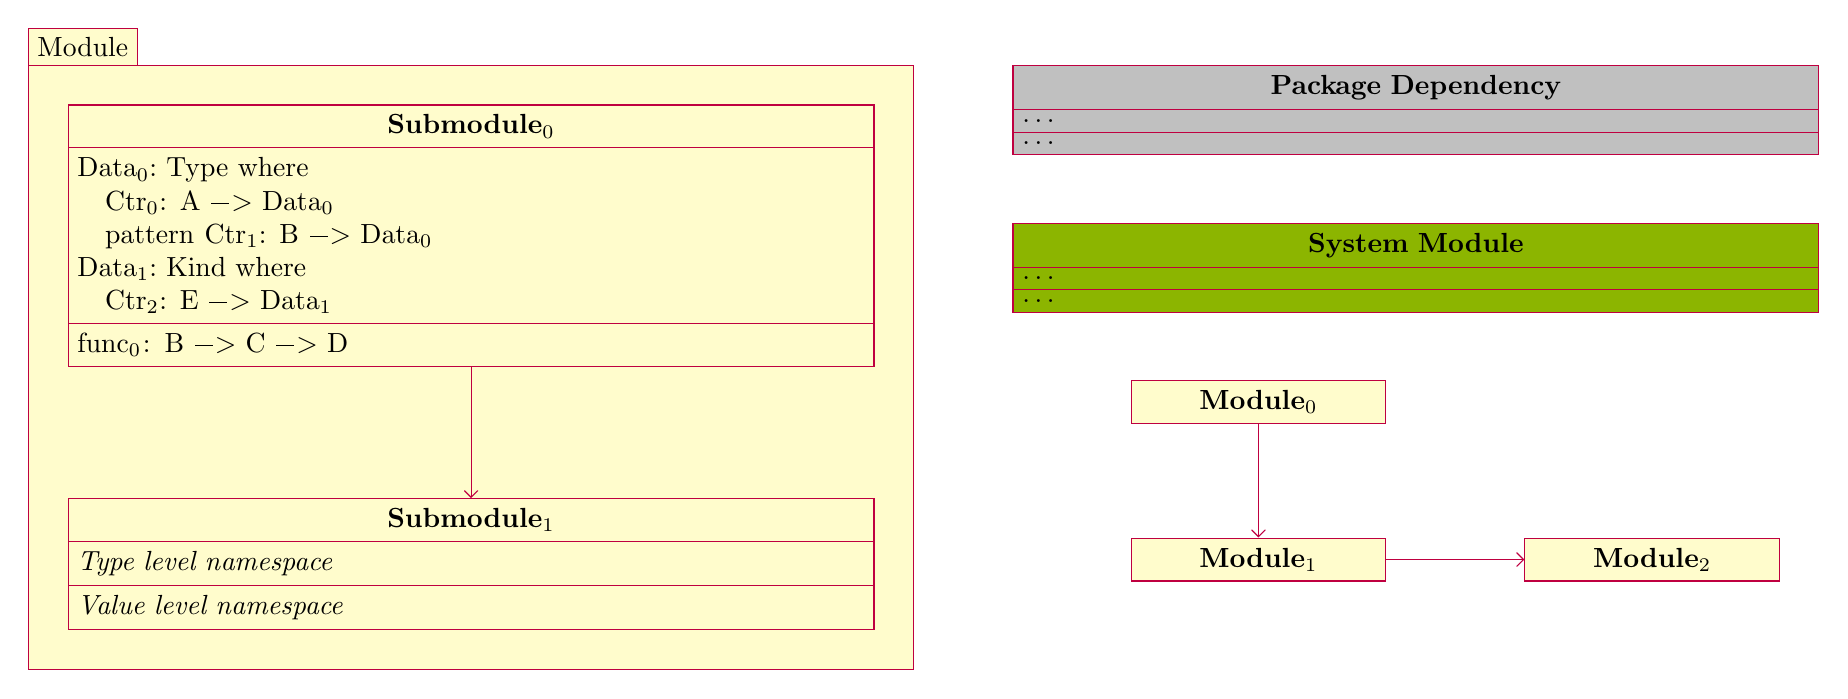
\begin{tikzpicture}

\begin{package}{Module}

\begin{class}[text width=10cm]{Submodule$_0$}{0,0}
\hstype{Data$_0$ : Type where}
\hstypectr{Ctr$_0$ : A -> Data$_0$}
\hstypectr{pattern Ctr$_1$ : B -> Data$_0$}
\hsfunc{func$_0$ : B -> C -> D} 
\hstype{Data$_1$ : Kind where}
\hstypectr{Ctr$_2$ : E -> Data$_1$}
\end{class}

\begin{class}[text width=10cm]{Submodule$_1$}{0,-5}
\attribute{\emph{Type level namespace}}
\operation{\emph{Value level namespace}}
\end{class}

\draw [umlcd style, ->] (Submodule$_0$.south) -- (Submodule$_0$ |- 
Submodule$_1$.north); 
\end{package}

\begin{class}[text width=3cm]{Module$_0$}{10,-3.5}
\end{class}

\begin{class}[text width=3cm]{Module$_1$}{10,-5.5}
\end{class}

\begin{class}[text width=3cm]{Module$_2$}{15,-5.5}
\end{class}

\draw [umlcd style, ->] (Module$_0$.south) -- (Module$_0$ |- 
Module$_1$.north); 
\draw [umlcd style, ->] (Module$_1$.east) -- (Module$_1$ -| 
Module$_2$.west); 

\renewcommand{\umlfillcolor}{grey}
\begin{class}[text width=10cm]{Package Dependency}{12,0.5}
\hstype{$\ldots$}
\hsfunc{$\ldots$}
\end{class}


\renewcommand{\umlfillcolor}{applegreen}
\begin{class}[text width=10cm]{System Module}{12,-1.5}
\hstype{$\ldots$}
\hsfunc{$\ldots$}
\end{class}

\end{tikzpicture}
}}\caption{Example of module diagram syntax}\label{fig:ModExample}
\end{figure}



\section{A Description of Module Diagram Syntax}\label{subsec:ModuleSyntax}

The module hierarchy is broken down into multiple levels to better describe the
system.  A coarse module hierarchy is given, and each module is further broken
into submodules.  A dependency between two modules $A$ and $B$ indicates that
each submodule in $A$ depends on all of $B$. There is no necessity to break
down modules into submodule, if they do not have any interesting submodule 
structure. Arrows between modules and submodules denote a dependency. 

External dependencies, which are modules which come from an external package,
are indicated in {\color{grey}grey}. System modules, which are modules part of
Ampersand, but not written specifically for EFA (or, on which EFA depends, but
few or no changes have been made from the original module before the existence
of EFA), are indicated in {\color{applegreen}green}. The module hierarchy of
these modules is not described here; they are included simply to indicate which
symbols are imported from these modules. An example of the syntax is found in
figure~\ref{fig:ModExample}.

\section{Module Hierarchy}\label{subsec:modhierarchy}

This section contains a hierarchical breakdown of each module, as well as a brief
explanation of each modules' elements. The module hierarchy of EFA as a whole 
is 
given in figure~\ref{fig:efaMod}.  Note
that every module which is part of EFA depends on the Haskell \texttt{base} 
package
(which is the core libraries of Haskell). Also note that for the \texttt{base}
package, we only include primitive definitions (i.e. those not defined in real
Haskell) which may be difficult to track down in the documentation. The kinds
\lstinline{Nat} and \lstinline{Symbol} correspond to type level natural number 
and string
literals, respectively. The kind \lstinline{Constraint} is the kind of class and
equality constraints, for example, things like \lstinline{Show x} and 
\lstinline[mathescape]|Int $\sim$ Bool|.  
Note that \texttt{Show} itself does \emph{not} have kind Constraint --
its kind is \lstinline{Type -> Constraint}. The detailed semantics of these
primitive entities can be found in the GHC user
guide~\cite{ghcUserGuide}. While
many modern features of GHC are used in the actual implementation, they are not
mentioned in, nor required to understand, the module description.

%% %% All other features of GHC are
%% %% detailed in the user guide as well, but no other

The primary interface to EFA is the function \lstinline{eca2PrettySQL}, which 
takes an FSpec (the abstract syntax of Ampersand) and an ECA rule, and returns 
the pretty
printed SQL code for that rule. Also note that while the dependencies within EFA
modules \edchange{WK}{is}{are} relatively complex, they depend on the rest of the Ampersand system
in a simple manner. The modules \lstinline{Test} and \lstinline{Prototype} 
implement the testing
framework and the prototype generation, respectively; these modules depend
directly on only one module from EFA, namely \lstinline{ECA2SQL}. Similarly, the
majority of EFA itself does not depend directly on Ampersand modules outside of
EFA. This makes EFA very resilient to changes in the core Ampersand system; in
order to update EFA to work with a modification to Ampersand, only one EFA
module -- ECA2SQL -- will generally need to be modified. 

All functions named in the module hierarchy are total - they do not throw
exceptions, or produce errors which are not handled or infinite loops. 
Therefore, no
additional information past the type of the function is required to deduce the
inputs and outputs of the function -- they are precisely the inputs and outputs
of the type.

\begin{figure}[!ht]
\makebox[\textwidth][c]{
\scalebox{0.6}{
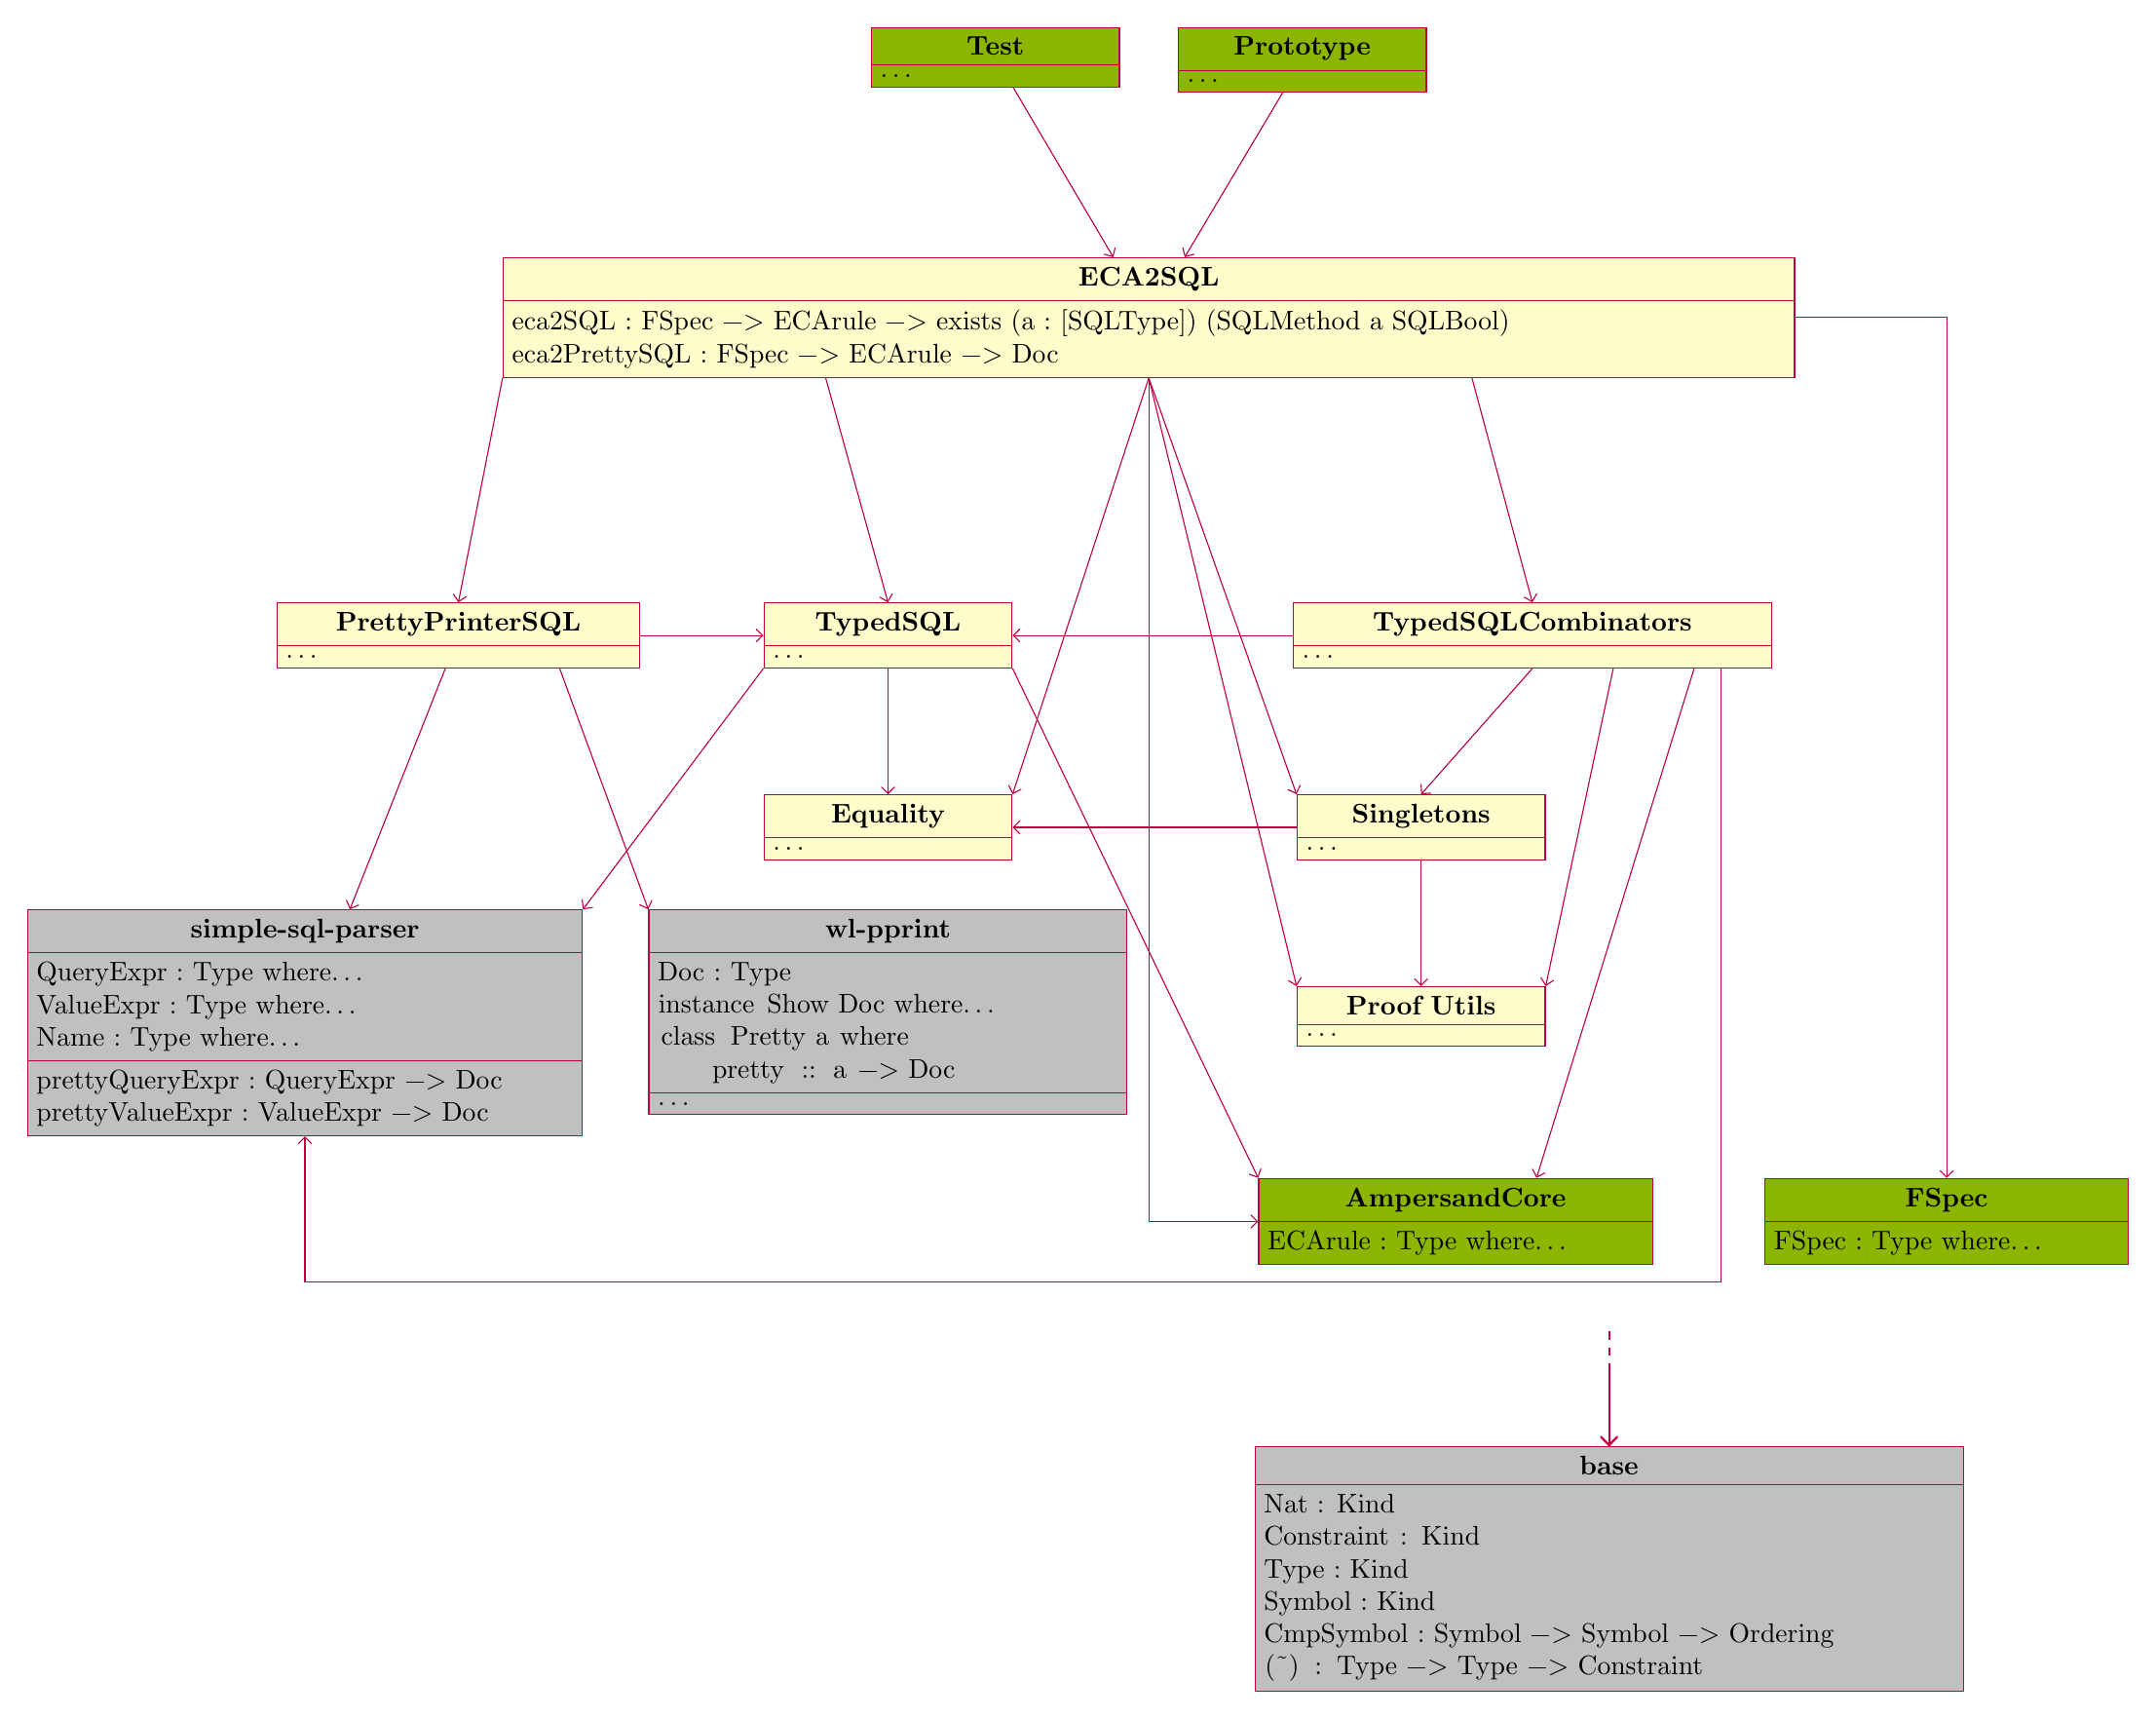
\begin{tikzpicture}

%% \begin{package}{TypedSQL}
%% fwQcGWGGF

\begin{class}[text width=16.6cm]{ECA2SQL}{0,2}
\hsfunc{eca2SQL : FSpec -> ECArule -> exists (a : [SQLType]) 
(SQLMethod a SQLBool)}
\hsfunc{eca2PrettySQL : FSpec -> ECArule -> Doc}
%% \hsfunc{$\ldots$}
\end{class}

\begin{class}[text width=3cm]{TypedSQL}{-3.4, -2.5}
\hsfunc{$\ldots$}
\end{class}

\begin{class}[text width=4.5cm]{PrettyPrinterSQL}{-9, -2.5}
\hsfunc{$\ldots$}
\end{class}

\begin{class}[text width=6cm]{TypedSQLCombinators}{5,-2.5}
\hsfunc{$\ldots$}
\end{class}


\begin{class}[text width=3cm]{Equality}{-3.4,-5}
\hsfunc{$\ldots$}
\end{class}

\begin{class}[text width=3cm]{Singletons}{3.55,-5}
\hsfunc{$\ldots$}
\end{class}


%% \begin{class}[text width=3cm]{Trace}{-3.4,-13.5}
%%     \hsfunc{$\ldots$}
%% \end{class}

\begin{class}[text width=3cm]{Proof Utils}{3.55,-7.5}
\hsfunc{$\ldots$}
\end{class}

\renewcommand{\umlfillcolor}{grey}
\begin{class}[text width=9cm]{base}{6,-13.5}
\hstype{Nat : Kind} 
\hstype{Constraint : Kind} 
\hstype{Type : Kind} 
\hstype{Symbol : Kind}
\hstype{CmpSymbol : Symbol -> Symbol -> Ordering} 
\hstype{(\~) : Type -> Type -> Constraint} 
\end{class}

\renewcommand{\umlfillcolor}{grey}
\begin{class}[text width=6cm]{wl-pprint}{-3.4,-6.5}
\hstype{Doc : Type} 
\hstype{instance Show Doc where $\ldots$} 
\hstype{class Pretty a where}
\hstype[20pt]{pretty :: a -> Doc}
\hsfunc{$\ldots$}
\end{class}

\renewcommand{\umlfillcolor}{grey}
\begin{class}[text width=7cm]{simple-sql-parser}{-11,-6.5}
\hstype{QueryExpr : Type where $\ldots$}
\hstype{ValueExpr : Type where $\ldots$}
\hstype{Name : Type where $\ldots$}
\hsfunc{prettyQueryExpr : QueryExpr -> Doc} 
\hsfunc{prettyValueExpr : ValueExpr -> Doc} 
\end{class}


\renewcommand{\umlfillcolor}{applegreen}
\begin{class}[text width=4.9cm]{AmpersandCore}{4,-10}
\hstype{ECArule : Type where $\ldots$} 
%% \hsfunc{$\ldots$}
\end{class}

\renewcommand{\umlfillcolor}{applegreen}
\begin{class}[text width=3cm]{Test}{-2,5}
\hsfunc{$\ldots$}
\end{class}

\renewcommand{\umlfillcolor}{applegreen}
\begin{class}[text width=3cm]{Prototype}{2,5}
\hsfunc{$\ldots$}
\end{class}

\renewcommand{\umlfillcolor}{applegreen}
\begin{class}[text width=4.5cm]{FSpec}{10.4,-10}
\hstype{FSpec : Type where $\ldots$} 
%% \hsfunc{$\ldots$}
\end{class}

\unidirectionalAssociation{Prototype}{}{}{ECA2SQL}
\unidirectionalAssociation{Test}{}{}{ECA2SQL}

\draw [umlcd style, ->] ($(ECA2SQL.south)!0.5!(ECA2SQL.south 
west)$) -- (TypedSQL.north); 
\draw [umlcd style, ->] ($(ECA2SQL.south)!0.5!(ECA2SQL.south 
east)$) -- (TypedSQLCombinators.north); 
\draw [umlcd style, ->] (ECA2SQL.south) -- (Equality.north east); 
\draw [umlcd style, ->] (ECA2SQL.south) -- (Singletons.north west); 
%% \draw [umlcd style, ->] (ECA2SQL.south) -- (Trace.north east); 
\draw [umlcd style, ->] (ECA2SQL.south) -- (Proof Utils.north 
west); 
\draw [umlcd style, ->] (ECA2SQL.south west) -- 
(PrettyPrinterSQL.north); 


\node[above = 1cm of base] (basedummy)       {};
\node[above = 1.5cm of base](basedummy2)       {};
\draw [umlcd style, ->, thick] (basedummy) -- (base); 
\draw [umlcd style dashed line, -, thick] (basedummy2) -- (base); 

\draw [umlcd style, ->] (Singletons.south) -- (Proof Utils.north); 
%% \draw [umlcd style, ->] (Singletons.west) -- (Trace.east); 
\draw [umlcd style, ->] (TypedSQL.south) -- (Equality.north); 
%% \draw [umlcd style, ->] (Equality.south) -- (Trace.north); 
\draw [umlcd style, ->] (TypedSQLCombinators.west) -- 
(TypedSQL.east); 
\draw [umlcd style, ->] (Singletons.west) -- (Equality.east); 
%% \draw [umlcd style, ->] (Proof Utils.south west) -- (Trace.south 
%%east); 
\draw [umlcd style, ->] (TypedSQL.south east) -- 
(AmpersandCore.north west); 

\draw [umlcd style, ->] ([xshift=60pt]TypedSQLCombinators.south) -- 
([xshift=30pt]AmpersandCore.north); 
\draw [umlcd style, ->] (TypedSQLCombinators.south) -- 
(Singletons.north); 
\draw [umlcd style, ->] ([xshift=30pt]TypedSQLCombinators.south) -- 
(Proof Utils.north east); 


\draw [umlcd style, ->] ([xshift=-30pt]PrettyPrinterSQL.south east) 
-- (wl-pprint.north west); 
%% \draw [umlcd style, ->] (PrettyPrinterSQL.south east) -- 
%%(Trace.west); 
\draw [umlcd style, ->] (PrettyPrinterSQL.east) -- (TypedSQL.west); 

%% \node[above = 1cm of Trace] (tracedummy)       {};
%% \node[above = 1.5cm of Trace](tracedummy2)       {};
%% \draw [umlcd style, ->, thick] (tracedummy) -- (Trace); 
%% \draw [umlcd style dashed line, -, thick] (tracedummy2) -- 
%%(Trace); 

\draw [umlcd style, ->] (TypedSQL.south west) -- 
(simple-sql-parser.north east); 

\draw  [umlcd style, ->, fill opacity=0]  
([xshift=70pt]TypedSQLCombinators.south) --++ (0cm,-8cm) -| 
(simple-sql-parser.south);


\draw[umlcd style ,->, fill opacity=0] (ECA2SQL.east) -| node[above 
, sloped , black]{} (FSpec.north);

\draw[umlcd style ,->, fill opacity=0] (ECA2SQL.south) |- 
node[above , sloped , black]{} (AmpersandCore.west);

\unidirectionalAssociation{PrettyPrinterSQL}{}{}{simple-sql-parser}

\end{tikzpicture}
}}\caption{Module diagram for EFA as a whole} \label{fig:efaMod}
\end{figure}


\FloatBarrier

\begin{figure}[!ht]
\makebox[\textwidth][c]{
\scalebox{0.6}{
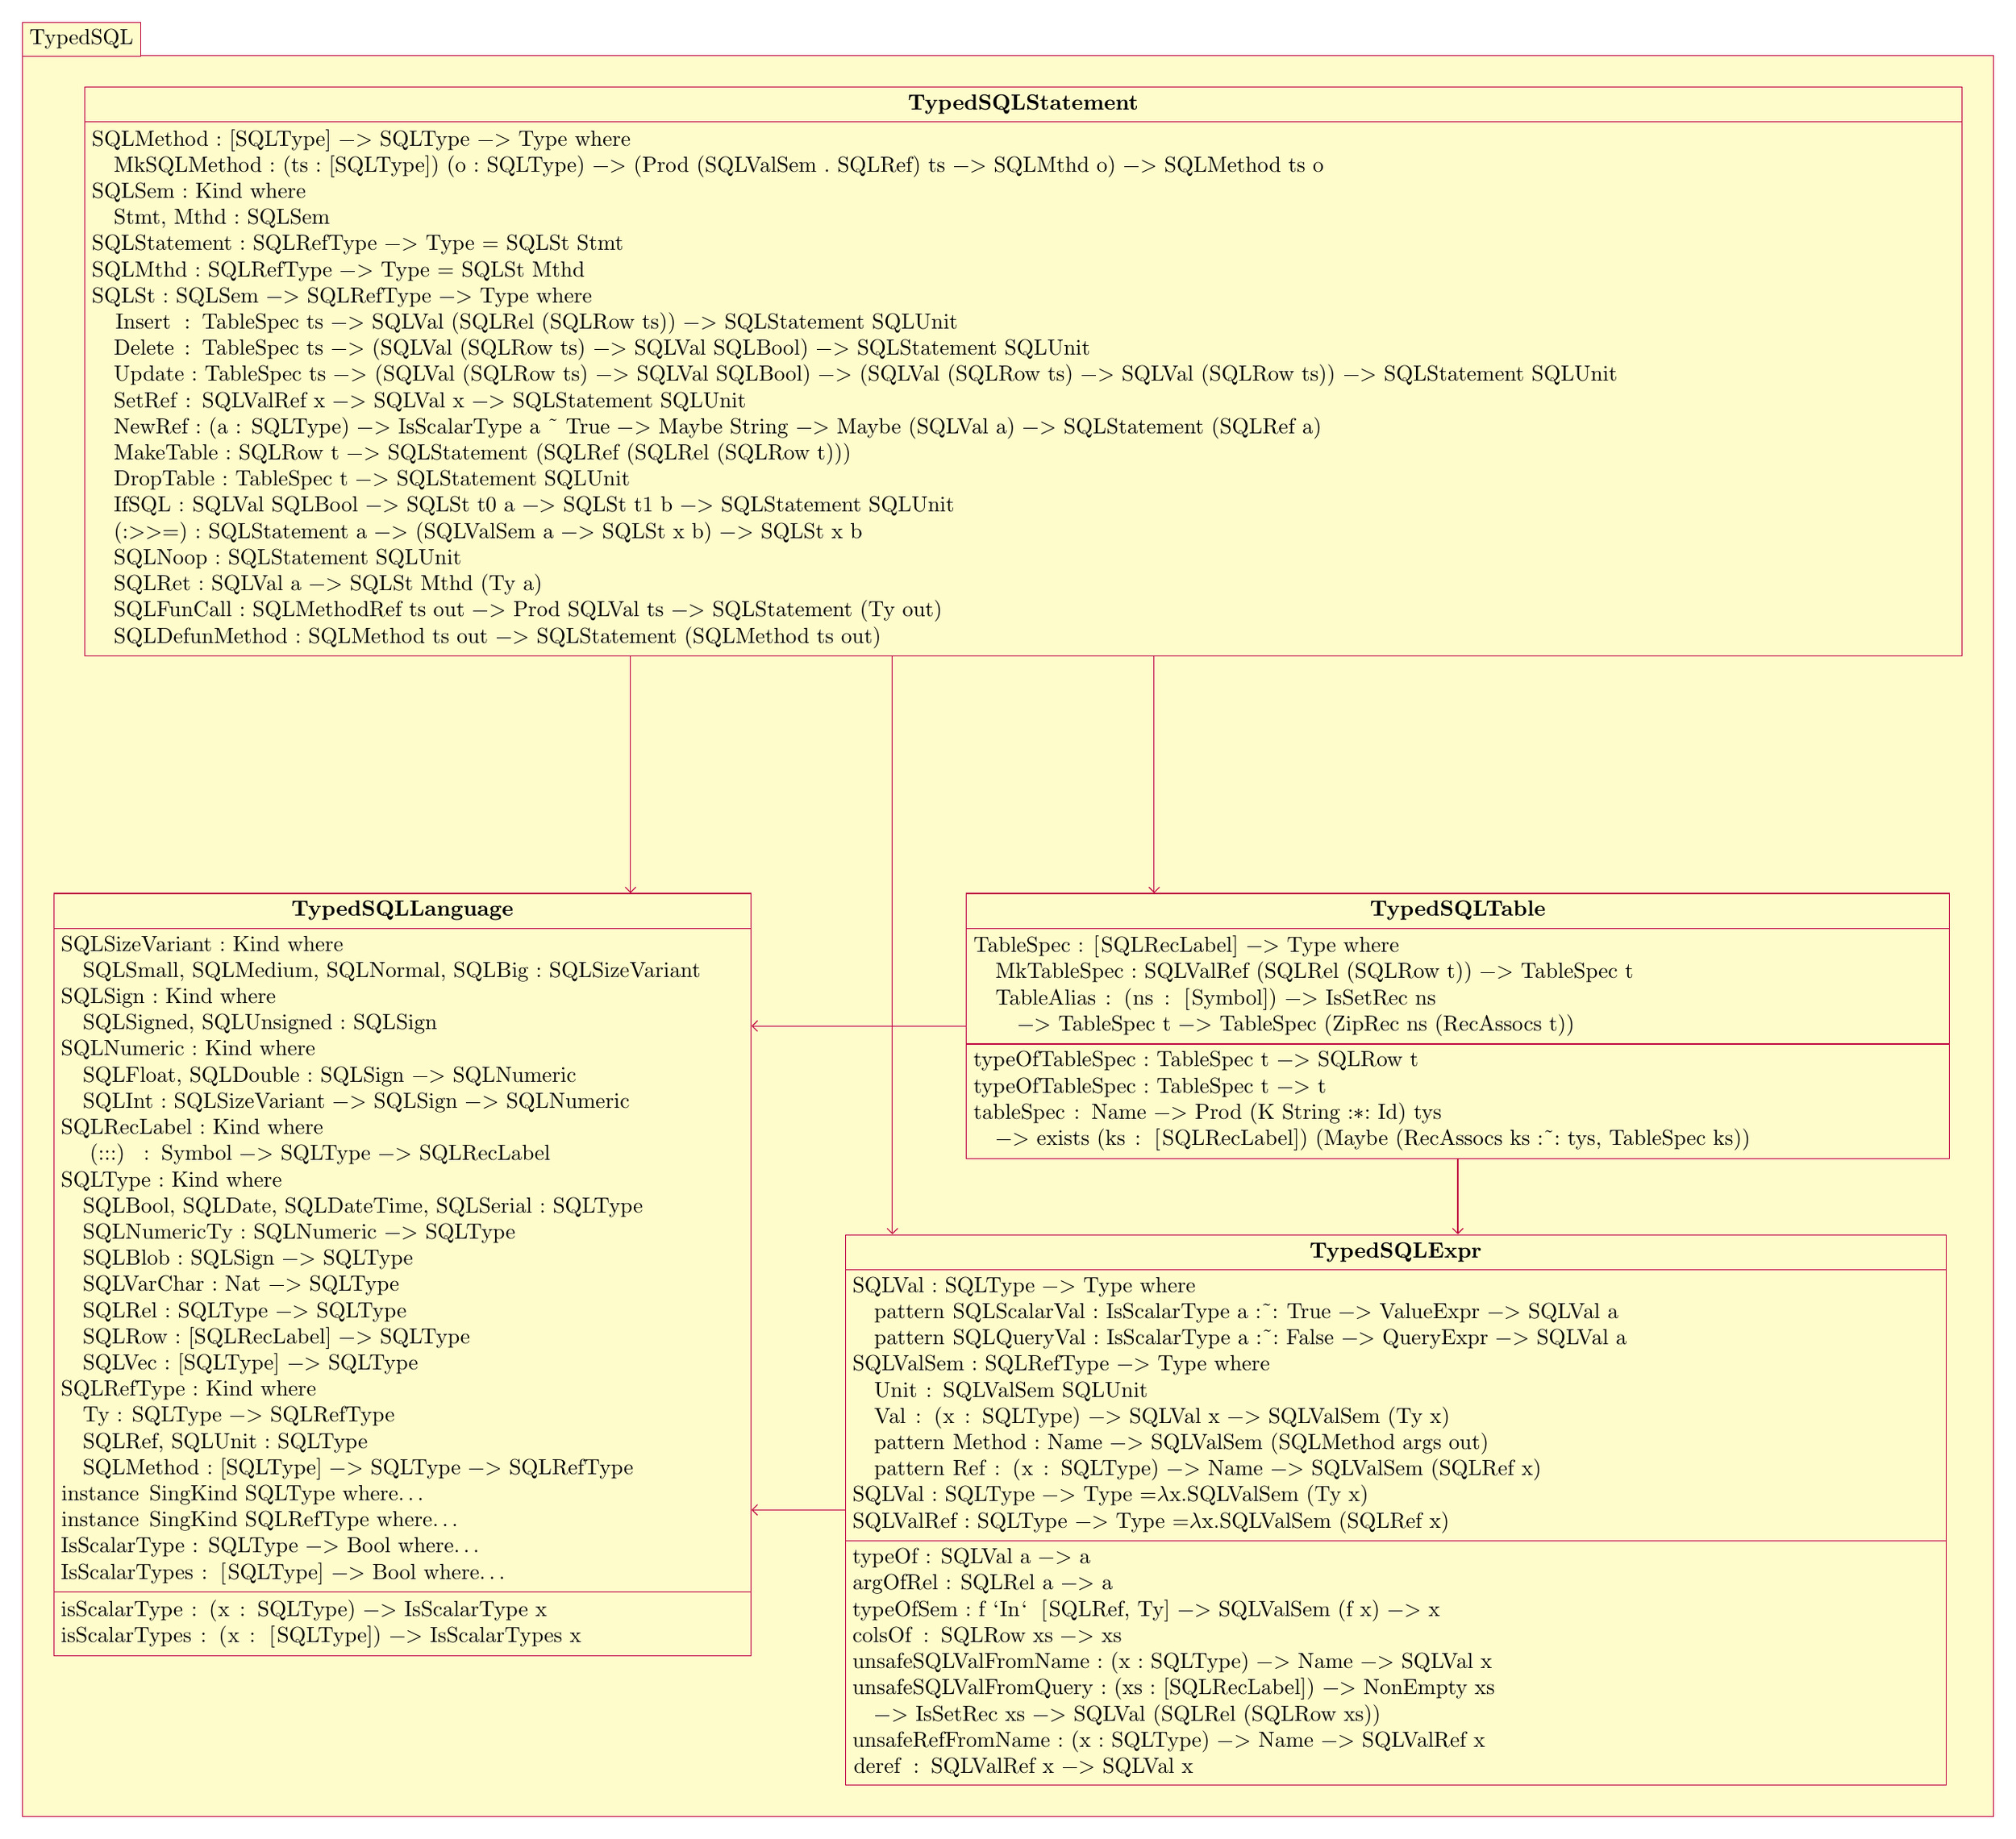
\begin{tikzpicture}

\begin{package}{TypedSQL}

\begin{class}[text width=30cm]{TypedSQLStatement}{10,18}
\hstype{SQLMethod : [SQLType] -> SQLType -> Type where}
\hstypectr{MkSQLMethod : (ts : [SQLType]) (o : SQLType) -> (Prod 
(SQLValSem . SQLRef) ts -> SQLMthd o) -> SQLMethod ts o}
%% \hstype[20pt]{-> (Prod (SQLValSem . SQLRef) ts -> SQLMthd o) -> 
%%SQLMethod ts o}

\hstype{SQLSem : Kind where}
\hstypectr{Stmt, Mthd : SQLSem}

\hstype{SQLStatement : SQLRefType -> Type = SQLSt Stmt}
\hstype{SQLMthd : SQLRefType -> Type = SQLSt Mthd}

\hstype{SQLSt : SQLSem -> SQLRefType -> Type where} 
\hstypectr{Insert : TableSpec ts -> SQLVal (SQLRel (SQLRow ts)) -> 
SQLStatement SQLUnit}
\hstypectr{Delete : TableSpec ts -> (SQLVal (SQLRow ts) -> SQLVal 
SQLBool) -> SQLStatement SQLUnit}
\hstypectr{Update : TableSpec ts -> (SQLVal (SQLRow ts) -> SQLVal 
SQLBool) -> (SQLVal (SQLRow ts) -> SQLVal (SQLRow ts)) -> 
SQLStatement SQLUnit}
\hstypectr{SetRef : SQLValRef x -> SQLVal x -> SQLStatement SQLUnit}
\hstypectr{NewRef : (a : SQLType) -> IsScalarType a \~ True -> 
Maybe String -> Maybe (SQLVal a) -> SQLStatement (SQLRef a)}
\hstypectr{MakeTable : SQLRow t -> SQLStatement (SQLRef (SQLRel 
(SQLRow t)))}
\hstypectr{DropTable : TableSpec t -> SQLStatement SQLUnit}
\hstypectr{IfSQL : SQLVal SQLBool -> SQLSt t0 a -> SQLSt t1 b -> 
SQLStatement SQLUnit}
\hstypectr{(:>>=) : SQLStatement a -> (SQLValSem a -> SQLSt x b) -> 
SQLSt x b}
\hstypectr{SQLNoop : SQLStatement SQLUnit}
\hstypectr{SQLRet : SQLVal a -> SQLSt Mthd (Ty a)}
\hstypectr{SQLFunCall : SQLMethodRef ts out -> Prod SQLVal ts -> 
SQLStatement (Ty out)}
\hstypectr{SQLDefunMethod : SQLMethod ts out -> SQLStatement 
(SQLMethod ts out)}
\end{class}


\begin{class}[text width=11cm]{TypedSQLLanguage}{0,5}   
\hstype{SQLSizeVariant : Kind where}
\hstypectr{SQLSmall, SQLMedium, SQLNormal, SQLBig : SQLSizeVariant}

\hstype{SQLSign : Kind where}
\hstypectr{SQLSigned, SQLUnsigned : SQLSign}

\hstype{SQLNumeric : Kind where}
\hstypectr{SQLFloat, SQLDouble : SQLSign -> SQLNumeric}
\hstypectr{SQLInt : SQLSizeVariant -> SQLSign -> SQLNumeric}

\hstype{SQLRecLabel : Kind where}
\hstypectr{(:::) : Symbol -> SQLType -> SQLRecLabel}

\hstype{SQLType : Kind where}
\hstypectr{SQLBool, SQLDate, SQLDateTime, SQLSerial : SQLType}
\hstypectr{SQLNumericTy : SQLNumeric -> SQLType}
\hstypectr{SQLBlob : SQLSign -> SQLType}
\hstypectr{SQLVarChar : Nat -> SQLType}
\hstypectr{SQLRel : SQLType -> SQLType}
\hstypectr{SQLRow : [SQLRecLabel] -> SQLType}
\hstypectr{SQLVec : [SQLType] -> SQLType}

\hstype{SQLRefType : Kind where}
\hstypectr{Ty : SQLType -> SQLRefType}
\hstypectr{SQLRef, SQLUnit : SQLType}
\hstypectr{SQLMethod : [SQLType] -> SQLType -> SQLRefType}

\hstype{instance SingKind SQLType where $\ldots$}
\hstype{instance SingKind SQLRefType where $\ldots$}

\hstype{IsScalarType : SQLType -> Bool where $\ldots$}
\hstype{IsScalarTypes : [SQLType] -> Bool where $\ldots$}

\hsfunc{isScalarType : (x : SQLType) -> IsScalarType x}
\hsfunc{isScalarTypes : (x : [SQLType]) -> IsScalarTypes x}
\end{class}


\begin{class}[text width=17.5cm]{TypedSQLExpr}{16,-0.5}
\hstype{SQLVal : SQLType -> Type where}
\hstypectr{pattern SQLScalarVal : IsScalarType a :\~: True -> 
ValueExpr -> SQLVal a}
\hstypectr{pattern SQLQueryVal  : IsScalarType a :\~: False -> 
QueryExpr -> SQLVal a}

\hsfunc{typeOf : SQLVal a -> a}
\hsfunc{argOfRel : SQLRel a -> a} 

\hstype{SQLValSem : SQLRefType -> Type where}
\hstypectr{Unit : SQLValSem SQLUnit}
\hstypectr{Val : (x : SQLType) -> SQLVal x -> SQLValSem (Ty x)}
\hstypectr{pattern Method : Name -> SQLValSem (SQLMethod args out)}
\hstypectr{pattern Ref : (x : SQLType) -> Name -> SQLValSem (SQLRef 
x)}

\hstype{SQLVal : SQLType -> Type = $\lambda$ x $.$ SQLValSem (Ty x)}
\hstype{SQLValRef : SQLType -> Type = $\lambda$ x $.$ SQLValSem 
(SQLRef x)}

\hsfunc{typeOfSem : f `In` [SQLRef, Ty] -> SQLValSem (f x) -> x}

\hsfunc{colsOf : SQLRow xs -> xs}

\hsfunc{unsafeSQLValFromName : (x : SQLType) -> Name -> SQLVal x}
\hsfunc{unsafeSQLValFromQuery : (xs : [SQLRecLabel]) -> NonEmpty xs}
\hsfunc[10pt]{ -> IsSetRec xs -> SQLVal (SQLRel (SQLRow xs))}
\hsfunc{unsafeRefFromName : (x : SQLType) -> Name -> SQLValRef x}

\hsfunc{deref : SQLValRef x -> SQLVal x}   
\end{class}


\begin{class}[text width=15.6cm]{TypedSQLTable}{17,5}
\hstype{TableSpec : [SQLRecLabel] -> Type where}
\hstypectr{MkTableSpec : SQLValRef (SQLRel (SQLRow t))  -> 
TableSpec t}
\hstypectr{TableAlias : (ns : [Symbol]) -> IsSetRec ns }
\hstype[20pt]{-> TableSpec t -> TableSpec (ZipRec ns (RecAssocs t))}

\hsfunc{typeOfTableSpec : TableSpec t -> SQLRow t}
\hsfunc{typeOfTableSpec : TableSpec t -> t}

\hsfunc{tableSpec : Name -> Prod (K String :*: Id) tys}
\hsfunc[10pt]{ -> exists (ks : [SQLRecLabel]) (Maybe (RecAssocs ks 
:\~: tys, TableSpec ks))}

\end{class}

\draw [umlcd style, ->] ([xshift=-60pt]TypedSQLStatement.south) -- 
([xshift=-60pt]TypedSQLStatement |- TypedSQLExpr.north); 
\draw [umlcd style, ->] ([xshift=60pt]TypedSQLStatement.south) -- 
([xshift=60pt]TypedSQLStatement |- TypedSQLTable.north); 
\draw [umlcd style, ->] ([xshift=-180pt]TypedSQLStatement.south) -- 
([xshift=-180pt]TypedSQLStatement |- TypedSQLLanguage.north); 


\draw [umlcd style, ->] (TypedSQLTable.south) -- (TypedSQLTable |- 
TypedSQLExpr.north); 
\draw [umlcd style, ->] (TypedSQLTable.west) -- (TypedSQLTable -| 
TypedSQLLanguage.east); 
\draw [umlcd style, ->] (TypedSQLExpr.west) -- (TypedSQLExpr -| 
TypedSQLLanguage.east);

\end{package}

\end{tikzpicture}
}}\caption{Module diagram for TypedSQL} \label{fig:typedSQL}
\end{figure}


\subsection{TypedSQL}

The module hierarchy for the TypedSQL module is shown in
figure \ref{fig:typedSQL}. The submodules of TypedSQL are quite large, 
however, the majority of the definitions within are type and kind definitions, 
which correspond precisely to entities defined by MySQL. The only exception is 
SQLRel, which distinguishes relations from scalar types - MySQL does not make 
this \edchange{WK}{distinguishment}{distinction}. 
Only a few
helper functions are defined in these modules -- namely, only things which 
form
the core interface to TypedSQL and in particular, SQLStatement. These 
functions
cannot be defined outside of the module, usually because they use an 
abstract
constructor. By making the core interface to TypedSQL very small, 
maintaining 
the TypedSQL language definition separately from the implementation of 
EFA is simplified. All of the data types in TypedSQL are correct by 
construction, with the exception of the functions explicitly labeled 
``unsafe''. These functions (unsafeSQLValFromName, unsafeSQLValFromQuery, and 
unsafeRefFromName)
are required only when implementing a new SQL primitive on top of the SQL
language - they are not intended for regular use. 

The TypedSQLLanguage module models the SQL type language in Haskell with a
series of kind declarations. The language being modeled is only a subset of 
the
SQL type language, corresponding approximately to the subset which the core
Ampersand system already uses. The meaning of each Haskell type corresponds
exactly to the appropriate MySQL type, which are detailed in the MySQL
manual \citep{mySQLman}. Similarly, the constructors of SQLSt all correspond
to different varieties of SQL statements -- for the majority of 
constructors,
there is a one-to-one correspondence between the semantics of the 
constructor,
and the semantics of the SQL statement with the same name. The exceptions 
are:     
\begin{description}
\item[\texttt{SQLNoop}] MySQL does not have a primitive no-op statement
\item[\texttt{SQLDefunMethod}]  MySQL does not allow defining 
procedures within procedures; 
this constructor denotes that a method ``defined'' within another 
statement must 
first be loaded as a MySQL Stored Procedure \citep{mySQLman}.
\item[\texttt{:>>=}] This constructor corresponds to sequencing 
statements. This constructor
embeds scope checking of MySQL statements in the Haskell compiler -- 
ill-formed statements
containing variables which are not defined (i.e. not in scope) will be 
rejected by the Haskell
compiler. 
\end{description}

The SQLSt data type also distinguishes between two varieties of statements:
SQLStatement and SQLMthd. The former is the type of regular statements, 
while the latter is the type of ``almost'' complete methods - methods whose 
formal parameters have not yet been bound. This is done in order to statically
guarantee that a SQL method always returns a value. Due to the type of
\lstinline{:>>=}, this also rules out SQL programs which contain dead code -- no
code can follow SQLRet, which is always guaranteed to return from the 
function.
While this does rule out some valid programs (for example, an if statement 
in
which both branches end with a return, but there is no return following the 
if
statement, will be rejected), these programs can be written in an equivalent
way in our language without any loss of generality.    

\subsection{TypedSQLCombinators}

The module TypedSQLCombinators, whose members are given in 
figure~\ref{fig:typedSQLComb},
implements a subset of primitive SQL functions on top of the TypedSQL 
expression type. 
The data type PrimSQLFunction encodes the specification of each 
function; the type
and semantics of each function is that of the corresponding function in 
MySQL (refer to
the MySQL manual ~\cite{mySQLman} for details on each function). The 
only exception
is the \lstinline{Alias} function, which is a primitive syntactic 
constructor (not a named entity)
in MySQL - rows can be aliased with a select statement. Aliasing a row 
means to change
the name of each association in the row, but not the shape of the row 
(i.e. the types of
each element of the row, as well as their ordering). The single 
function \lstinline{primSQL}
implements all of the primitive SQL functions. It takes as an argument 
a specification
of the primitive function, a tuple of arguments of the correspond 
types, and returns
a SQL value, again of the corresponding type. 

\begin{figure}[!ht]
    \makebox[\textwidth][c]{
        \scalebox{0.6}{
            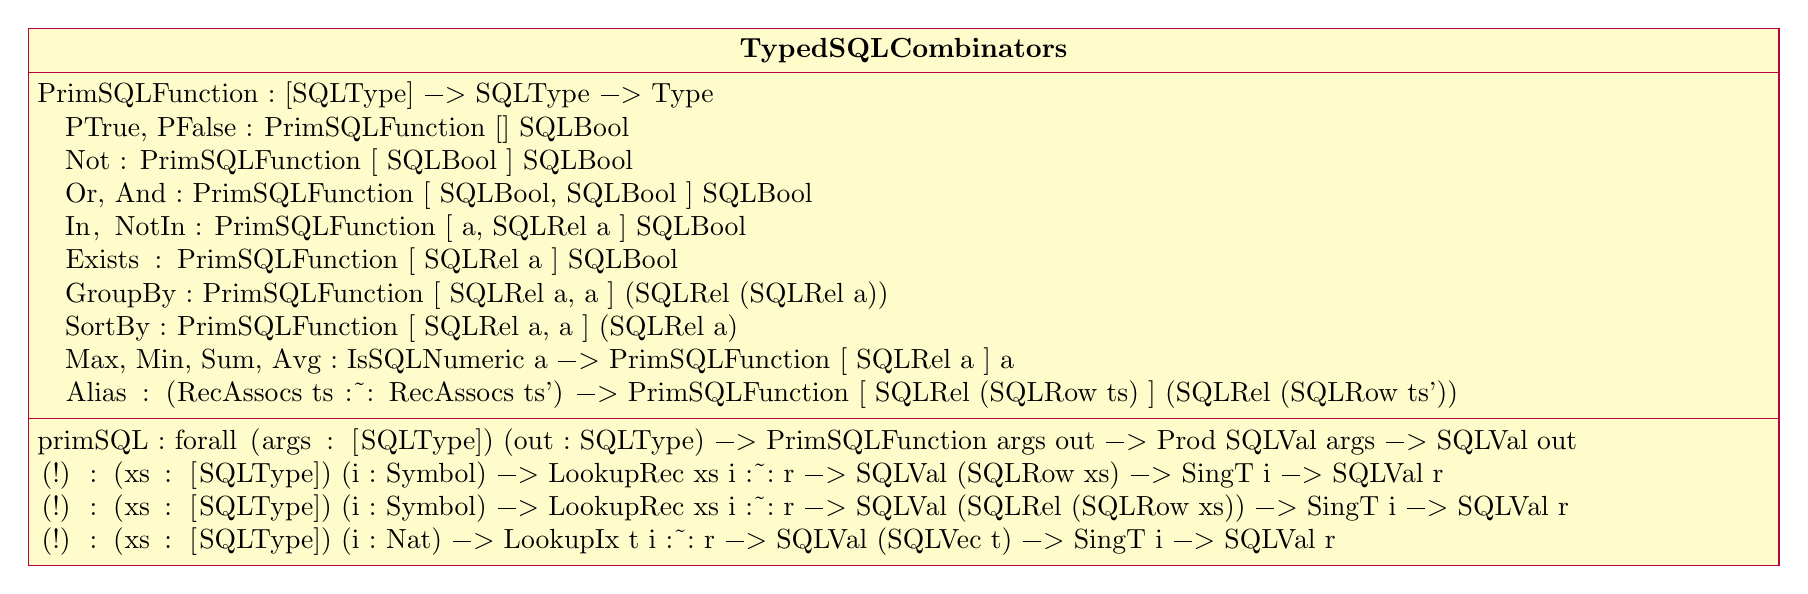
\begin{tikzpicture}
            
            %% \begin{package}{TypedSQL}
            \begin{class}[text width=22cm]{TypedSQLCombinators}{17,5}
            \hstype{PrimSQLFunction : [SQLType] -> SQLType -> Type}
            \hstypectr{PTrue, PFalse : PrimSQLFunction [] SQLBool}
            \hstypectr{Not : PrimSQLFunction [ SQLBool ] SQLBool}
            \hstypectr{Or, And : PrimSQLFunction [ SQLBool, SQLBool ] 
                SQLBool}
            \hstypectr{In, NotIn : PrimSQLFunction [ a, SQLRel a ] SQLBool}
            \hstypectr{Exists : PrimSQLFunction [ SQLRel a ] SQLBool}
            \hstypectr{GroupBy : PrimSQLFunction [ SQLRel a, a ] (SQLRel 
                (SQLRel a))}
            \hstypectr{SortBy  : PrimSQLFunction [ SQLRel a, a ] (SQLRel a)}
            \hstypectr{Max, Min, Sum, Avg : IsSQLNumeric a -> 
                PrimSQLFunction [ SQLRel a ] a }
            \hstypectr{Alias : (RecAssocs ts :~: RecAssocs ts') -> 
                PrimSQLFunction [ SQLRel (SQLRow ts) ] (SQLRel (SQLRow ts'))}
            
            \hsfunc{primSQL : forall (args : [SQLType]) (out : SQLType) -> 
                PrimSQLFunction args out -> Prod SQLVal args -> SQLVal out}
            
            \hsfunc{(!) : (xs : [SQLType]) (i : Symbol) -> LookupRec xs i 
                :\~: r -> SQLVal (SQLRow xs) -> SingT i -> SQLVal r}
            \hsfunc{(!) : (xs : [SQLType]) (i : Symbol) -> LookupRec xs i 
                :\~: r -> SQLVal (SQLRel (SQLRow xs)) -> SingT i -> SQLVal r}
            \hsfunc{(!) : (xs : [SQLType]) (i : Nat) -> LookupIx t i :\~: r 
                -> SQLVal (SQLVec t) -> SingT i -> SQLVal r}
            
            
            \end{class}
            
            %% \end{package}
            
            \end{tikzpicture}
        }}\caption{Module diagram for TypedSQLCombinators} 
        \label{fig:typedSQLComb}
\end{figure}





\begin{figure}[!ht]
\makebox[\textwidth][c]{
    \scalebox{0.6}{
        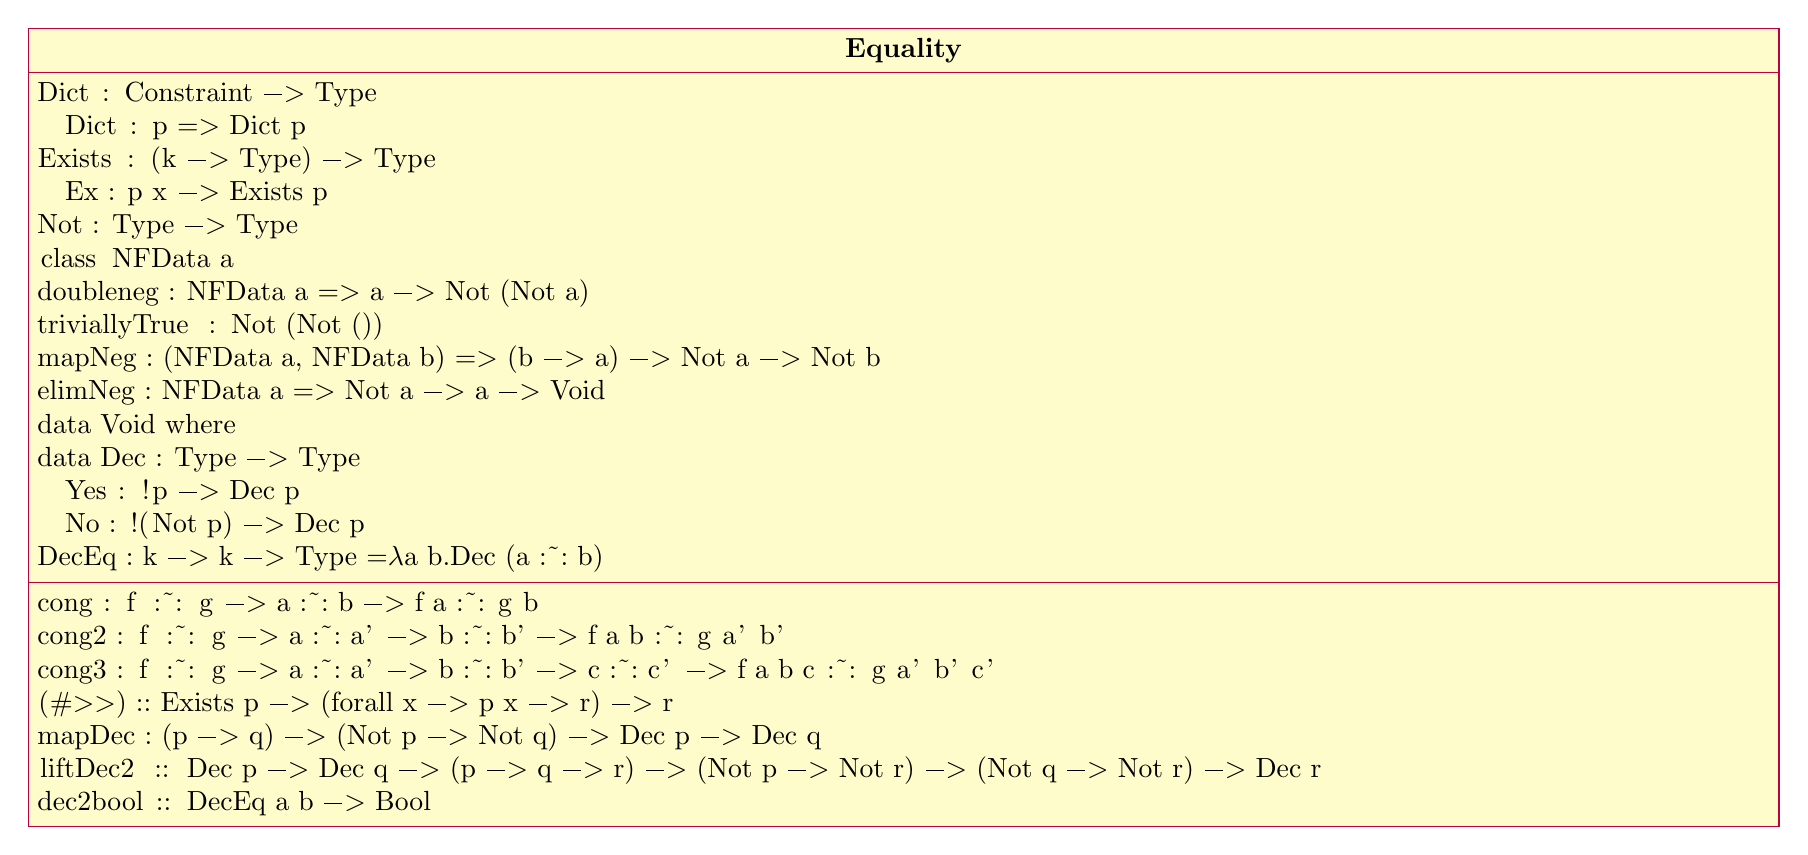
\begin{tikzpicture}
        
        \begin{class}[text width=22cm]{Equality}{17,5}
        
        \hsfunc{cong : f :\~: g -> a :\~: b -> f a :\~: g b}
        \hsfunc{cong2 : f :\~: g -> a :\~: a' -> b :\~: b' 
        -> f a b :\~: g a' b'}
        \hsfunc{cong3 : f :\~: g -> a :\~: a' -> b :\~: b' 
        -> c :\~: c' -> f a b c :\~: g a' b' c'}
        
        \hstype{Dict : Constraint -> Type}
        \hstypectr{Dict : p => Dict p}
        
        \hstype{Exists : (k -> Type) -> Type} 
        \hstypectr{Ex : p x -> Exists p}
        
        \hsfunc{($\#$>>) :: Exists p -> (forall x -> p x -> 
        r) -> r}
        
        \hstype{Not : Type -> Type} 
        
        \hstype{class NFData a}
        
        \hstype{doubleneg : NFData a => a -> Not (Not a)} 
        
        %% Why is this particular defintion off by about 
        %%2pt? Very strange...
        \hstype[-2pt]{triviallyTrue : Not (Not ())}
        
        \hstype{mapNeg : (NFData a, NFData b) => (b -> a) 
        -> Not a -> Not b}
        
        \hstype{elimNeg : NFData a => Not a -> a -> Void}
        
        \hstype{data Void where}
        
        \hstype{data Dec : Type -> Type}
        \hstypectr{Yes : !p -> Dec p}
        \hstypectr{No  : !(Not p) -> Dec p}
        
        \hstype{DecEq : k -> k -> Type = $\lambda$ a b$.$ 
        Dec (a :\~: b)}
        
        \hsfunc{mapDec : (p -> q) -> (Not p -> Not q) -> 
        Dec p -> Dec q}
        
        \hsfunc{liftDec2 :: Dec p -> Dec q -> (p -> q -> r) 
        -> (Not p -> Not r) -> (Not q -> Not r) -> Dec r}
        
        \hsfunc{dec2bool :: DecEq a b -> Bool}
        
        \end{class}
        
        \end{tikzpicture}
    }}\caption{Module diagram for Equality} 
    \label{fig:equality}
\end{figure}

\subsection{Equality}

The Equality module (\ref{fig:equality}) defines several 
utilities for working
with proof-like values, including the existential 
quantification data type,
proofs of congruence of propositional equality of various 
arities -- \lstinline{cong, cong2, cong3} -- and the Dec type, which 
encodes the concept of
a decidable proposition. The most important element of this 
module, however is
the abstract \lstinline{Not} type. We must prove certain 
things about our
program to the Haskell type system. For example, if one 
attempts to construct a
scalar SQLVal for some SQLType $S$, one must first prove 
that that type is a
scalar type. The main use of this is decidable equality, 
which is similar to
regular equality, but additionally to giving a ``yes'' or 
``no'' answer, it also
stores a \emph{proof} of that answer.

The view of propositions as types comes from the 
Curry-Howard
isomorphism \cite{props}; however, this is not quite sound 
in Haskell, because
every type is inhabited by $\bot$, which corresponds to 
\texttt{undefined}, an
exception, or non-termination. Due to laziness, an 
unevaluated $\bot$ can be
silently ignored. At worst, this corresponds to a sound use 
of
\lstinline{unsafeCoerce} leaking into the ``outside 
world'', that is, allowing
a user to accidently expose the use of an 
\lstinline{unsafeCoerce}. One can
usually work around this by evaluating all proof-like 
values to normal form
before working with them (this is accomplished by the 
\lstinline{NFData} class,
which stands for normal form data). The normal form of most 
datatypes contains
precisely one ``type'' of bottom -- namely the value 
$\bot$, as opposed to
$\bot$ wrapped in a constructor, for example 
\lstinline[mathescape=true]{Just $\bot$}. This
bottom can then be removed with the Haskell primitive 
\lstinline{seq},
producing a value which can soundly be used as a proof.

A problem arises when we consider the negation of a proposition. $\lnot p$ 
is typically encoded in Haskell as \lstinline[mathescape=true]{p -> $\bot$}, where the type 
$\bot$
can be represented by any uninhabited type, typically called\lstinline{Void}. 
However, the normal form of a function can contain any number of $\bot$ hidden 
deep inside the function, because evaluating a function to normal form only 
evaluates up to the outermost binder.
\edcomm{WK}{(You are aware of \texttt{deepseq}?)}
\edcomm{YT}{We are aware and do use it. Perhaps it should be added to the module diagram}
To prevent any
unsoundness which this might cause, values of type \lstinline{Not p} are reduced
to normal form as they are built, starting with a canonical value which is known
to be in normal form - the value \lstinline{triviallyTrue}.  This is the role of
NFData in the type signature of \lstinline{mapNeg}.  As mentioned previously,
the type \lstinline{Not} is abstract, so the provided interface, which is known
to be sound, is the only way to construct and eliminate values of type
\lstinline{Not p}.


\subsection{PrettySQL}

The module PrettySQL defines pretty printers for each of the types
corresponding to SQL entities, including SQL types, SQL values, SQL references
and methods, and SQL statements. These pretty printers produce a value of
type Doc (which comes from the wl-pprint package), which is like a string
, but contains the layout and indentation of all lines of the document,
allowing for easy composition of Doc values into larger documents, without
worrying about layout. The SQL entities are pretty printed in a human
readable format, complete with SQL comments which indicate the origin
and motive of generated code. 


\begin{figure}[!ht]
    \makebox[\textwidth][c]{
        \scalebox{0.6}{
            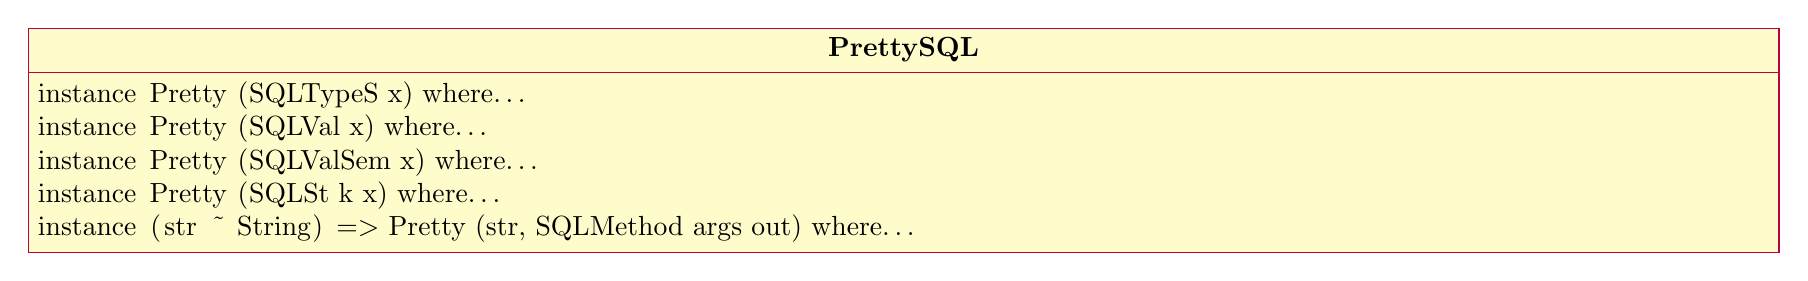
\begin{tikzpicture}
            
            \begin{class}[text width=22cm]{PrettySQL}{17,5}
            
            \hstype{instance Pretty (SQLTypeS x) $\,\,$ where 
                $\ldots$}
            \hstype{instance Pretty (SQLVal x)  $\,\,$ where 
                $\ldots$}
            \hstype{instance Pretty (SQLValSem x)  $\,\,$ where 
                $\ldots$}
            \hstype{instance Pretty (SQLSt k x)  $\,\,$ where 
                $\ldots$}
            \hstype{instance (str \~ String) => Pretty (str, 
                SQLMethod args out)  $\,\,$ where $\ldots$}
            
            \end{class}
            
            \end{tikzpicture}
        }}\caption{Module diagram for PrettySQL} 
        \label{fig:prettySQL}
    \end{figure}

\subsection{Proof Utils}

The ProofUtils modules, shown in 
figure~\ref{fig:utilsMod}, provides various
utilities for proving compile time invariants, 
including the definitions of
various predicates used in other modules, as well as 
the value-level functions
which prove or disprove those predicates. Generally 
speaking, a predicate is a
type level function which returns either a true or 
false value, or has kind
\lstinline{Constraint}, in which case truth corresponds 
to a satisfied
constraint, while false to an unsatisfied one. Many 
predicates have value level
witnesses as well; these are datatypes which are 
inhabited if and only if the
predicate is true.  Therefore, pattern matching on the 
predicate witness can be used to recover a proof of the predicate at run time.

The function of the most important predicates and types is briefly summarized 
as follows. 

\begin{figure}[!ht]
\makebox[\textwidth][c]{
    \scalebox{0.6}{
        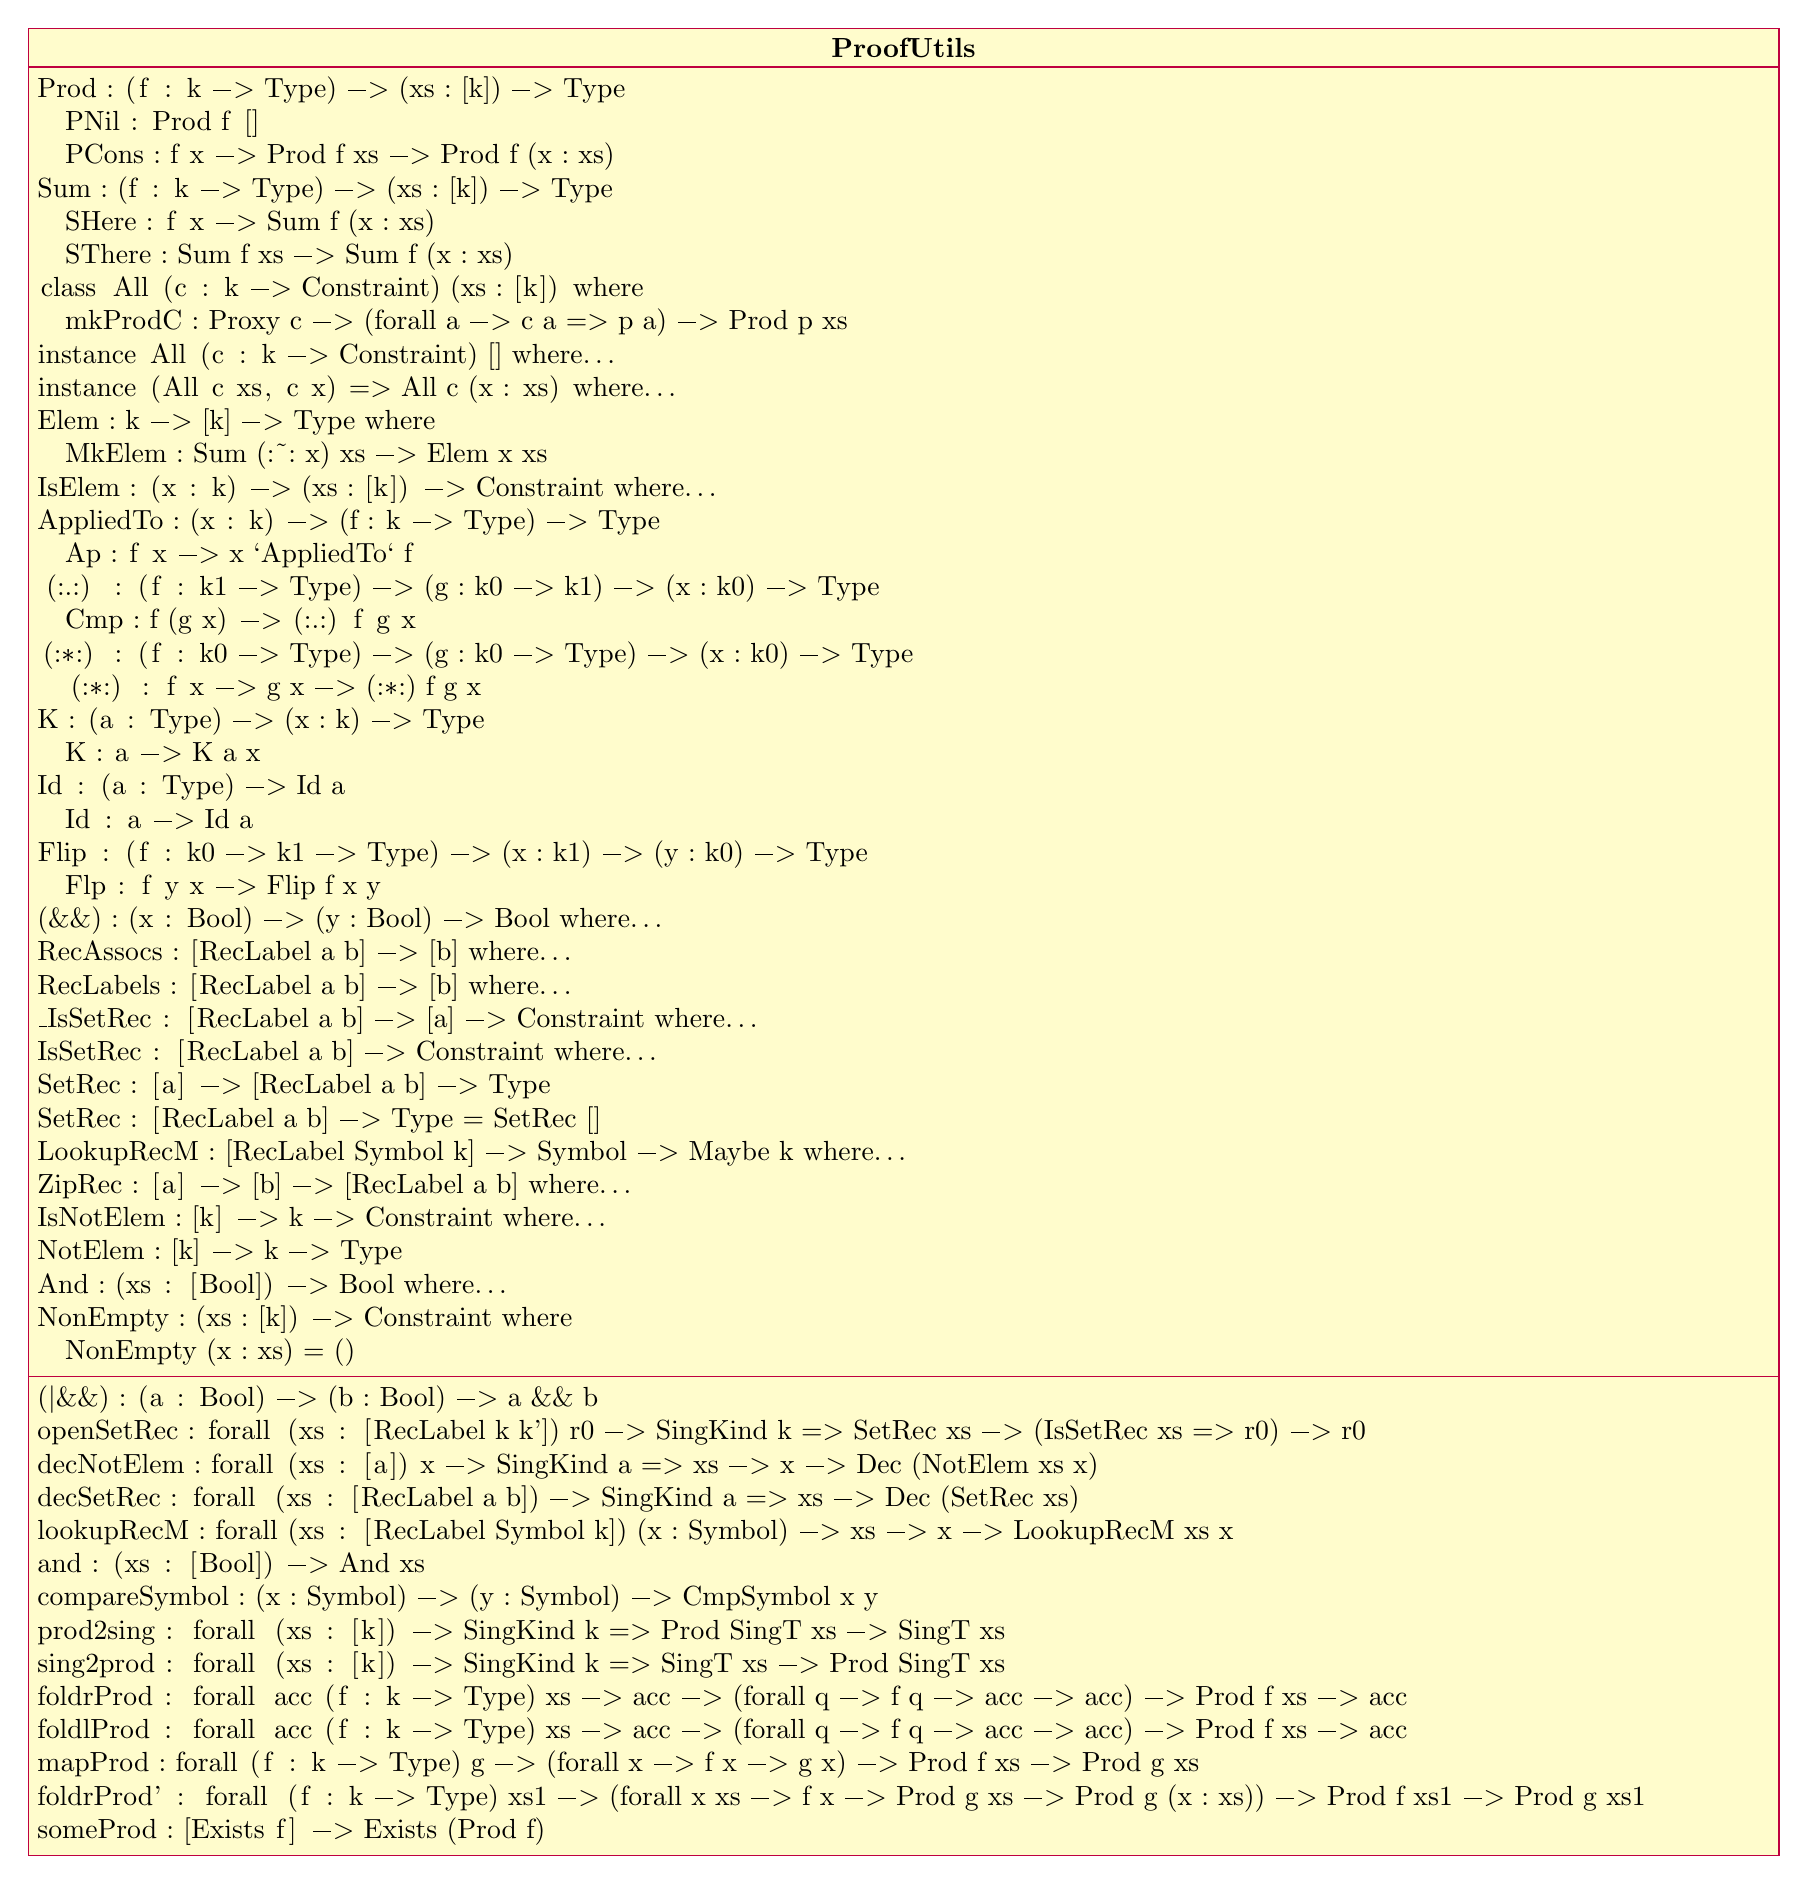
\begin{tikzpicture}
        
        \begin{class}[text width=22cm]{ProofUtils}{17,5}
        
        \hstype{Prod : (f : k -> Type) -> (xs : [k]) -> 
            Type} 
        \hstypectr{PNil : Prod f []}
        \hstypectr{PCons : f x -> Prod f xs -> Prod f 
            (x : xs)}
        
        \hstype{Sum : (f : k -> Type) -> (xs : [k]) -> 
            Type}  
        \hstypectr{SHere : f x -> Sum f (x : xs)}
        \hstypectr{SThere : Sum f xs -> Sum f (x : xs)}
        
        
        \hstype{class All (c : k -> Constraint) (xs : 
            [k]) where}
        \hstypectr{mkProdC : Proxy c -> (forall a -> c 
            a => p a) -> Prod p xs}
        
        \hstype{instance All (c : k -> Constraint) [] 
            where $\ldots$}
        \hstype{instance (All c xs, c x) => All c (x : 
            xs) where $\ldots$}
        
        \hstype{Elem : k -> [k] -> Type where}
        \hstypectr{MkElem : Sum (:\~: x) xs -> Elem x 
            xs} 
        
        \hstype{IsElem : (x : k) -> (xs : [k]) -> 
            Constraint where $\ldots$} 
        \hstype{AppliedTo : (x : k) -> (f : k -> Type) 
            -> Type}
        \hstypectr{Ap : f x -> x `AppliedTo` f}
        
        \hstype{(:.:) : (f : k1 -> Type) -> (g : k0 -> 
            k1) -> (x : k0) -> Type}
        \hstypectr{Cmp : f (g x) -> (:.:) f g x} 
        
        \hstype{(:*:) : (f : k0 -> Type) -> (g : k0 -> 
            Type) -> (x : k0) -> Type} 
        \hstypectr{(:*:) : f x -> g x -> (:*:) f g x} 
        \hstype{K : (a : Type) -> (x : k) -> Type} 
        \hstypectr{K : a -> K a x} 
        \hstype{Id : (a : Type) -> Id a}
        \hstypectr{Id : a -> Id a} 
        
        \hstype{Flip : (f : k0 -> k1 -> Type) -> (x : 
            k1) -> (y : k0) -> Type} 
        \hstypectr{Flp : f y x -> Flip f x y} 
        
        \hstype{(&&) : (x : Bool) -> (y : Bool) -> Bool 
            where $\ldots$} 
        
        \operation{\lstinline[mathescape]{(|&&) : (a : 
                Bool) -> (b : Bool) -> a && b}}
        
        \hstype{RecAssocs : [RecLabel a b] -> [b] where 
            $\ldots$} 
        \hstype{RecLabels : [RecLabel a b] -> [b] where 
            $\ldots$} 
        
        \hstype{IsSetRec\_ : [RecLabel a b] -> [a] -> 
            Constraint where $\ldots$} 
        
        \hstype{IsSetRec : [RecLabel a b] -> Constraint 
            where $\ldots$} 
        \hstype{SetRec\_ : [a] -> [RecLabel a b] -> 
            Type} 
        \hstype{SetRec : [RecLabel a b] -> Type = 
            SetRec\_ []} 
        
        
        \hsfunc{openSetRec : forall (xs : [RecLabel k 
            k']) $\,\,$r0 -> SingKind k => SetRec xs -> 
            (IsSetRec xs => r0) -> r0}
        
        \hsfunc{decNotElem : forall (xs : [a]) $\,\,$x 
            -> SingKind a => xs -> x -> Dec (NotElem xs x)}
        
        \hsfunc{decSetRec : forall (xs : [RecLabel a 
            b]) -> SingKind a => xs -> Dec (SetRec xs)}
        
        \hstype{LookupRecM : [RecLabel Symbol k] -> 
            Symbol -> Maybe k where $\ldots$} 
        
        \hsfunc{lookupRecM : forall (xs : [RecLabel 
            Symbol k]) (x : Symbol) -> xs -> x -> 
            LookupRecM xs x}
        
        \hstype{ZipRec : [a] -> [b] -> [RecLabel a b] 
            where $\ldots$} 
        
        \hstype{IsNotElem :  [k] -> k -> Constraint 
            where $\ldots$} 
        \hstype{NotElem : [k] -> k -> Type}
        
        \hstype{And : (xs : [Bool]) -> Bool where 
            $\ldots$} 
        
        \hsfunc{and\_t : (xs : [Bool]) -> And xs}
        
        \hsfunc{compareSymbol : (x : Symbol) -> (y : 
            Symbol) -> CmpSymbol x y}
        
        
        \hstype{NonEmpty : (xs : [k]) -> Constraint 
            where} 
        \hstypectr{NonEmpty (x : xs) = ()} 
        
        \hsfunc{prod2sing : forall (xs : [k]) -> 
            SingKind k => Prod SingT xs -> SingT xs} 
        \hsfunc{sing2prod : forall (xs : [k]) -> 
            SingKind k => SingT xs -> Prod SingT xs} 
        \hsfunc{foldrProd : forall acc (f : k -> 
            Type)$\,\,$xs -> acc -> (forall q -> f q -> acc 
            -> acc) -> Prod f xs -> acc}
        \hsfunc{foldlProd : forall acc (f : k -> 
            Type)$\,\,$xs -> acc -> (forall q -> f q -> acc 
            -> acc) -> Prod f xs -> acc}
        \hsfunc{mapProd : forall (f : k -> Type)$\,\,$g 
            -> (forall x -> f x -> g x) -> Prod f xs -> 
            Prod g xs}
        \hsfunc{foldrProd' : forall (f : k -> 
            Type)$\,\,$xs1 -> (forall x xs -> f x -> Prod g 
            xs -> Prod g (x : xs)) -> Prod f xs1 -> Prod g 
            xs1 }
        \hsfunc{someProd : [Exists f] -> Exists (Prod 
            f)}
        
        \end{class}
        
        \end{tikzpicture}
    }}\caption{Module diagram for ProofUtils} 
    \label{fig:utilsMod}
\end{figure}

\begin{description}
    \item[\texttt{Prod}] The type \lstinline{Prod f xs} 
    represents the $n$-ary product of the type
    level list $xs$, with each $x \in xs$ being mapped 
    to the type \lstinline{f x}. This 
    type is accompanied by the functions 
    \lstinline{prod2sing, sing2prod} which convert
    between singletons and products; the functions 
    \lstinline{foldrProd, foldlProd, foldrProd'}, 
    which are all eliminators for \lstinline{Prod} 
    (several eliminators are needed because the 
    most general eliminator is not well typed in 
    Haskell). 
    \item[\texttt{Sum}] The same as above, but the 
    $n$-ary sum as opposed to product. 
    \item[\texttt{All}] The constraint 
    \lstinline{All c xs} holds if and only if 
    \lstinline{c x} holds for 
    all $x \in xs$. 
    \item[\texttt{Elem, IsElem}]
    \lstinline{IsElem x xs} holds precisely when $x \in 
    xs$. 
    \lstinline{Elem} is the witness of 
    \lstinline{IsElem}. 
    \item[\texttt{AppliedTo, Ap, :.:, Cmp, :*:, K, Id, 
    Flip}] Categorical data types which encode
    a generalized view of algebraic data types. This 
    approach is largely standardized (and is only
    replicated here to avoid incurring a large 
    dependency) -- for more information, 
    see~\cite{alacarte}. 
    \item[\texttt{RecAssocs, RecLabels, ZipRec}] Type 
    level functions for working with type level 
    records. 
    A record in this context is a list of types of some 
    kind, each associated with a unique string label. 
    \lstinline{RecAssocs, RecLabels} retrieve the 
    associations and labels of a record, respectively, 
    while \lstinline{ZipRec} constructs such a record 
    from the associations and labels. It is the case
    that 
    \lstinline{ZipRec (RecAssocs x) (RecLabels x) == x} for all 
    \lstinline{x} .
    \item[\texttt{IsSetRec, SetRec}] The predicate 
    \lstinline{IsSetRec x} holds precisely if 
    \lstinline{x}
    is a valid record type, whose labels are all 
    unique. \lstinline{SetRec} is the witness for 
    \lstinline{IsSetRec}. 
    \item[\texttt{IsNotElem, NotElem}] The predicate 
    \lstinline{IsNotElem x xs} holds precisely if 
    $\lnot x \in xs$.
    \lstinline{NotElem} is the witnss for 
    \lstinline{IsNotElem}. 
    \item[\texttt{\&\&,And}] Binary and $n$-ary boolean 
    conjunction, with the usual semantics. 
\end{description}
    
    
\subsection{Singletons}\label{subsec:Singletons}

The Singletons module (figure ~\ref{fig:singletons}) is 
not fully detailed here; rather, a vastly simplified version is presented. The
\lstinline{SingT} type denotes a generic singleton for 
any kind which implements
\lstinline{SingKind} -- then, the main operation of 
interest on singletons is
decidable equality, which is realized by the function 
\lstinline{%==}. The
    detailed implementation is omitted because the 
    singletons approach in Haskell
    is well known and well 
    documented~\cite{singletons}. We re-implement
    singletons instead of using the well established 
    \texttt{singletons} library
    because, while this library is very well written, 
    it relies very heavily on
    Template Haskell~\cite{th}, which is essentially 
    string-based
    metaprogramming. Template Haskell is extremely 
    error prone and very difficult
    to maintain. As one of our primary goals is 
    long-term maintainability, and
    Template Haskell changes, sometimes drastically, 
    with every new release of
    GHC, including it in this project was deemed not 
    worth the
    headache. Therefore, we have reimplemented 
    singletons without Template
    Haskell, at the cost of having to write slightly 
    more boilerplate.


\begin{figure}[!ht]
    \makebox[\textwidth][c]{
        \scalebox{0.6}{
            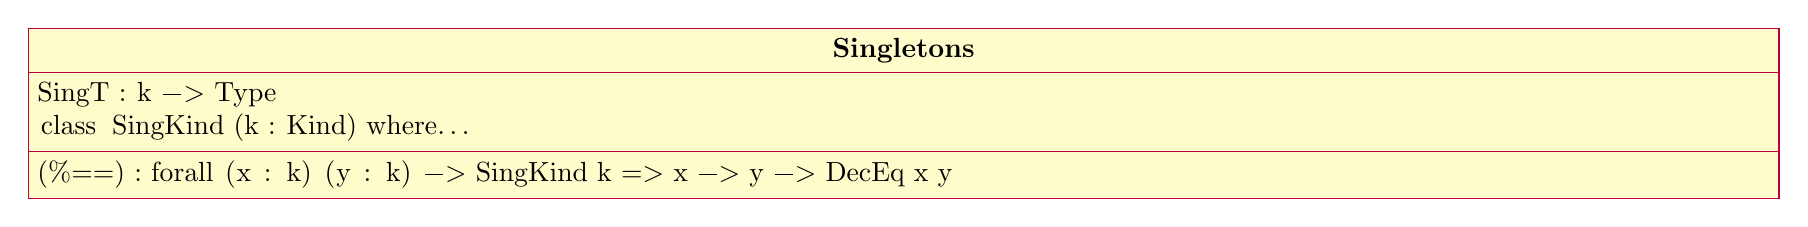
\begin{tikzpicture}
            
            \begin{class}[text width=22cm]{Singletons}{17,5}
            \hstype{SingT : k -> Type} 
            \hstype{class SingKind (k : Kind) where $\ldots$} 
            \hsfunc{(\%==) : forall (x : k) (y : k) -> SingKind k => x 
                -> y -> DecEq x y}
            
            \end{class}
            
            \end{tikzpicture}
        }}\caption{Module diagram for Singletons} \label{fig:singletons}
\end{figure}

\section{Key Algorithm}

This section contains the literate Haskell documentation of the portion 
of the EFA source code which implements the key algorithm of EFA. 

%% Assuming that `Capstone' and `ampersand' are in the same directory
%% and that there is a link from ECA2SQL.lhs -> ECA2SQL.tex 
\input{../../ampersand/src/Database/Design/Ampersand/ECA2SQL}

\edcomm{WK}{I guess this is an ancient fragment about AMMBR ---
prehaps better refer to section 1.3 for description of AMMBR.

Here, you probably want to talk about the algorithm
you use for translating ECA rules into SQL,
given the different ways Ampersand stores relations,
and the fact that ECA rules refer to relations, not tables.
}%edcomm

\section{Communication Protocol}

The EFA implementation needs to communicate with the front end to be able to 
run the generated SQL queries when a violation occurs.
\edcomm{WK}{It would probably be more precise to say that the SQL
fragments generated by EFA need to be invoked by the front end.}

\begin{itemize}
    \item \textbf{Old communication protocol -  PHP engine} \\
    In the existing version, Ampersand depends on PHP code to run the 
    generated SQL on the database. However, this comes at the cost of 
    human intervention, which results in manual maintenance when 
    changes occur during development.
    \edcomm{WK}{As such, putting SQL commands into generated PHP
    does not require human intervention --- they do it for testing,
    don't they?}
    \item \edinsert{WK}{\textbf{Current Ampersand development version:}
      All generated material is stored in JSON files --- these could
      also be used to store EFA-generated SQL. It is then up to the
      front-end implementation to connect them to violations.}
    \item \textbf{New Communication protocol - Stored Procedures} \\
    The developments teams of EFA has come to a conclusion that the 
    best way of communicating with the front-end will be to use Stored 
    Procedures\cite{SP}. These Stored Procedures provide the extra 
    benefit of query optimization at compile time which results in 
    better performance. While this is a suggested change, it will 
    require changes to the existing Ampersand software in order for 
    this idea to be successfully implemented. This anticipated 
    change will be implemented in the near future.
    
\end{itemize}

\chapter{Testing}

\edcomm{WK}{Here and also in other places it does get in the way
  of readability that Haskell is typographically not distinguished
  from text. (That's why I use \texttt{\backslash{}sf} in WKlhs.sty.)
}%edcomm
This chapter covers property testing using QuickCheck, system testing using a 
built-in test suite and MySQL WorkBench for SQL query testing. EFA's 
implementation uses dependent types which express application-specific program 
invariants that are beyond the scope of existing type systems. The tests that 
are implemented make two assumptions, the first being any element reused from 
the Ampersand system is already correct, and the second being that if the 
properties of a function are correctly implemented, when used in combination 
with assumption one that the outcome is correct.

\section{Property Testing Using QuickCheck}
Not all functions can be tested using QuickCheck due to their complexity (e.g. 
eca2SQL). All of EFA's modules rely on a few base modules, and testing the 
properties of the functions implemented in the base modules, by extension, 
tests all functions that rely on these core modules. These tests can be checked 
using stack and running \verb|``quickCheck <function>''|. The data types are 
presumed correct as they produce the correct results and are accepted by the 
Ampersand system. Furthermore, proof of EFA's TypedSQL was provided in software 
implementation section \ref{subsec:modhierarchy}.

\subsubsection*{Singletons.singKindWitness1}
For every pair of types and their type representation, an isomorphism exists,
\edcomm{WK}{This sounds very strange. In particular, the isomorphism
  is not specified to be related in any way to the quantified-over
  pair of types\ldots
  Any additional assumptions missing?
}%edcomm
where an isomorphism is a morphism $f:\ a \rightarrow b$ and there exists a
morphism $g: b \rightarrow a$ with $fg$ = $1_b$ and $gf$ = $1_a$. The default
implementation uses \lstinline{unsafeCoerce} and will only work if everything
is correctly defined.
         

\subsubsection*{Singletons.sing2val and Singletons.val2sing}
sing2val takes a singleton for some type and converts it to the value
from which it was promoted (e.g. \lstinline{'True} becomes \lstinline{True}).
val2sing does the opposite, except that it must return its output 
existentially quantified. These functions should be witnesses to the isomorphism
between singletons and their unlifted types, i.e it should be the case
that \lstinline{sing2val . val2sing = id} and \lstinline{val2sing . sing2val = id}. 


\subsubsection*{Singletons.$\boldsymbol{(\%==)}$} 
This function implements equality between types by induction on their singletons.
This function (when viewed as a binary relation) should be an equivalence, 
so therefore symmetry, transitive, and reflexive. 

\begin{description}[labelindent=1cm]
\item[Transitivity] $\forall\ a,\ b,\ c \in  X$ : ($aRb \wedge bRc$)$ \Rightarrow\ aRc$
\item[Reflexivity] $\forall a \in\ X $($aRa$)  
\item[Symmetry] $\forall a, b, \in X$ ($aRb \Rightarrow bRa$) 
\end{description}

\subsubsection*{Utils.foldrProd}
This function, and similarly \lstinline{Utils}.\lstinline{foldlProd} implement
the natural fold over the \lstinline{Prod} type, in the same way that 
the function \lstinline{foldr} acts upon lists. This function
must satisfy the property that it behaves the same as \lstinline{foldr}
does on lists. The function \lstinline{zipProd}, \lstinline{mapProd}, and \lstinline{foldlProd}
have similar properties. 


\subsection{System Testing Using Test suite}
The test suite is built using the Cabal build system and can be 
enabled by running \texttt{cabal configure --enable-tests} and
run by running the created test executable in the subfolder
\texttt{dist/build/ampersand-test/ampersand-test} of the 
project root directory. 

%% The test suite runs by using the cabal system and running 
\edcomm{YT}{Dont use `verb' unless you actually need verbatim text, use `texttt'}
%% \verb|``cabal configure --enable-tests''|; this test suite was built 
%% specifically for EFA and 
%% more details are provided in the 
\edcomm{YT}{Random link to random code? why}
%% \href{https://github.com/4ZP6Capstone2015/ampersand/blob/master/src/Database/Design/Ampersand/ECA2SQL/FreshName.lhs}{literate
 %% source code} located in EFA's github repository.

\section{Manual Execution of EFA's SQL Queries}

The queries produced by EFA were manually tested on a MySQL server; Ampersand 
relies on a MySQL database which can be installed as a part of xampp along with 
apache or simply on its own from the MySQL website~\cite{MySQL-web}. A simple guide is 
available on MySQL's website on how to install use WorkBench with xampp; if an 
MySQL server outside of xampp \edcomm{WK}{verb missing}, it is highly advisable for these two components 
to be installed together. Furthermore, WorkBench~\cite{workbench} can be found on 
MySQL's official website.

Xampp must be running Apache and MySQL for WorkBench to be able to connect to 
the database server. 
\begin{figure}[!h]
    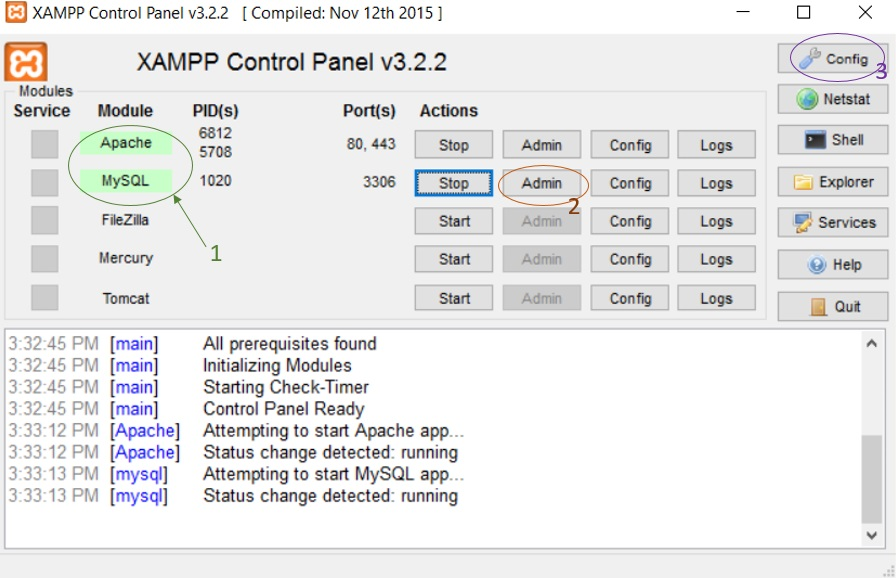
\includegraphics[width=\textwidth]{images/xampp}
    \caption{\footnotesize{1. Shows that both and Apache and MySQL must be 
    running at the same time. 2. The Admin button for mySQL opens phpAdmin 
    which is an graphical interface for accessing the databases in an MySQL 
    server. 3. Configuration button $\rightarrow$ services and ports 
    $\rightarrow$ [MySQL] tab, check that the port is identical to the 
    connected established for WorkBench. The standard is port 3306 }}
\end{figure}

Queries can be executed manually using WorkBench.
%% , to follow instructions on how 
%% to set up a connection for WorkBench, please refer to appendix 
%% \ref{appen:WorkBench}. 
Once WorkBench is running properly, it will look 
similar to the screen shot provided.
\begin{figure}[!h]
    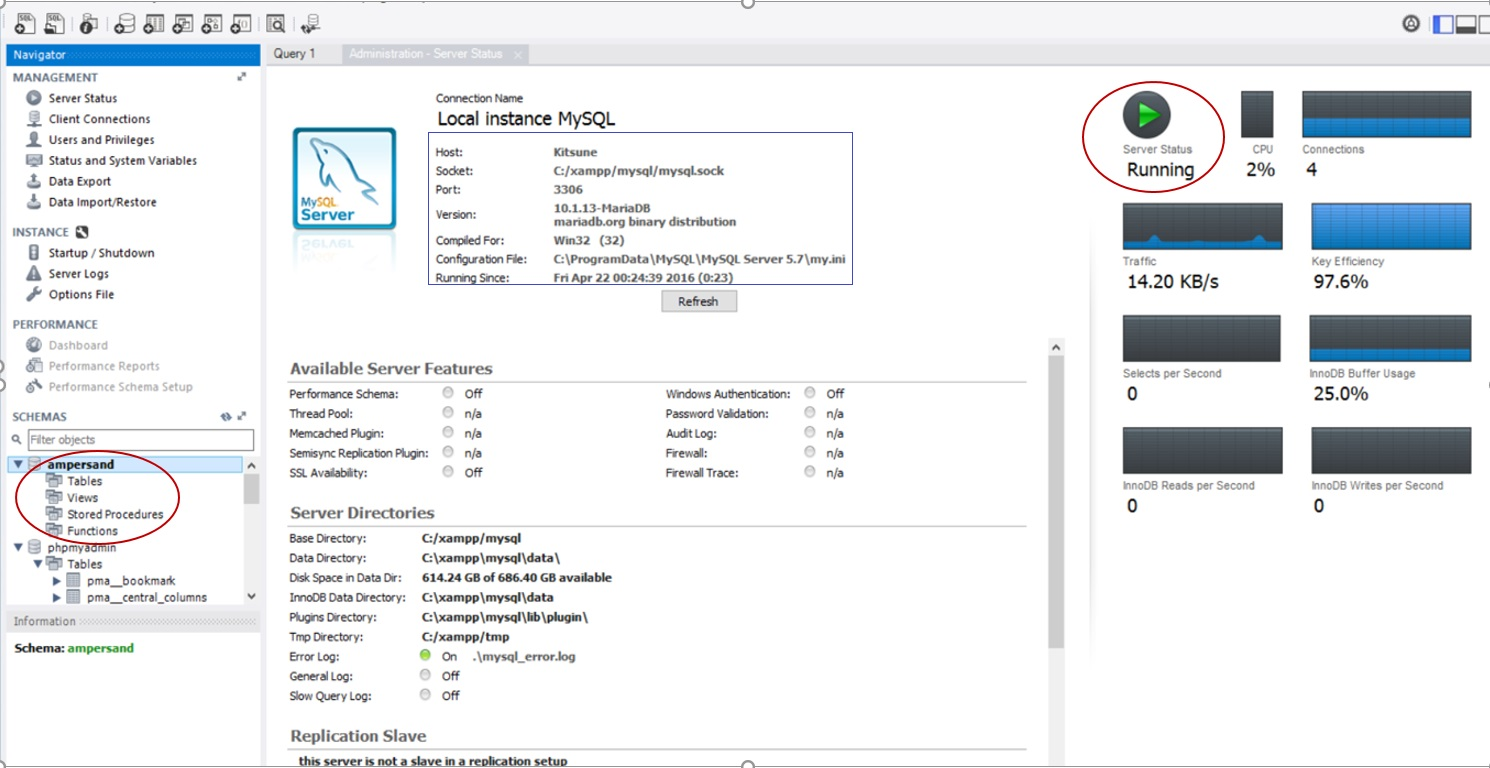
\includegraphics[width=\textwidth]{images/WorkBench}
    \caption{\footnotesize{The right-hand side shows the status of the server, 
    and on the lower left-hand side under `SCHEMAS', all the databases in 
    current server is listed. Ampersand requires a local database and a 
    password, both of which are `ampersand'. The blue box in the top middle 
    area provides information concerning the host. }}
\end{figure}

Queries are executed by going to [File] $\rightarrow$ [New Query Tab], a new 
tab will open and one can manually type queries. The execution of these queries 
can be specified to the highlighted portion or everything. The pretty-printer 
outputs onto the command console what is given as output to the Ampersand its 
database. 

\begin{figure}[!h]
    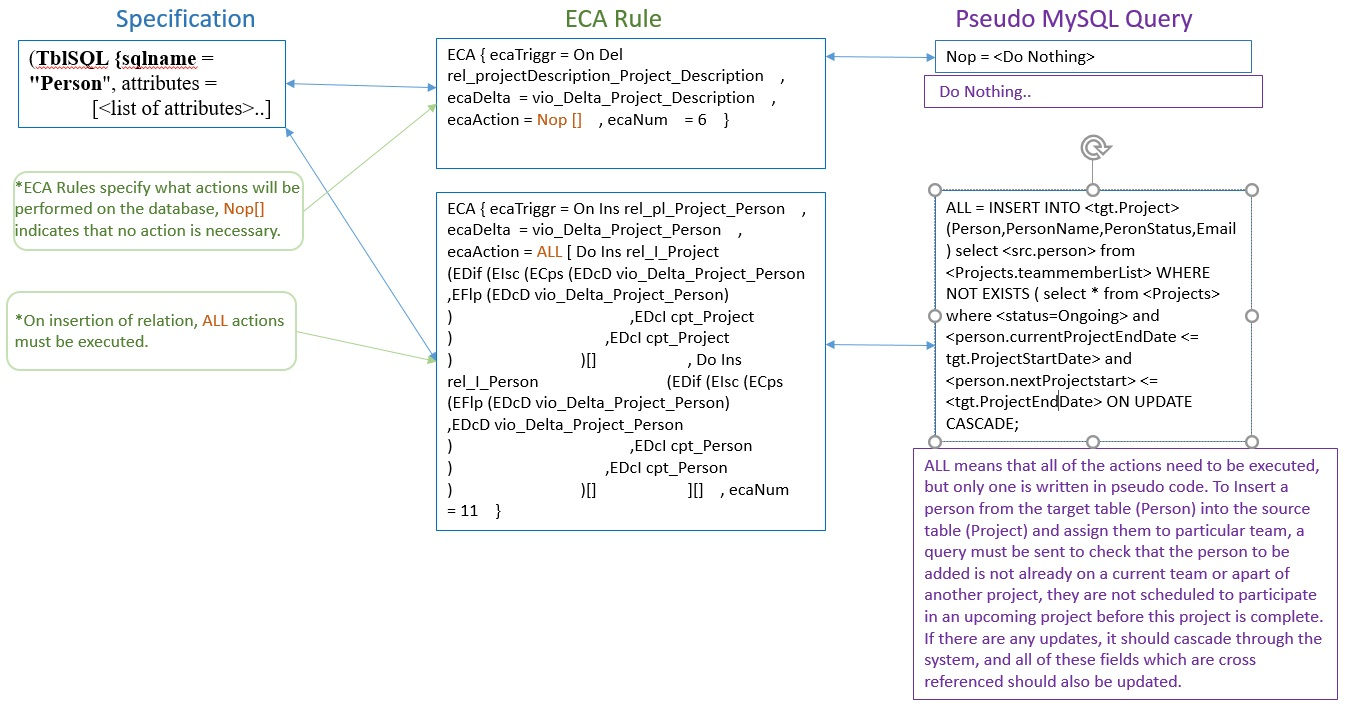
\includegraphics[width=\textwidth]{images/sqlquery}
    \caption{\footnotesize{This figure shows what the system sees in terms of 
    specification, how ECA are structured, and how they are to be executed in 
    SQL. }}
\end{figure}






\newpage

\bibliographystyle{alpha}
\bibliography{references}
\newpage
\section*{Appendix}
This section contains literate Haskell code and notes on implementation issues.
\subsection*{Literate Haskel Code}
%\include{Freshname}
\subsection*{Notes on Implementation Issues}

This section contains a detailed list of concerns that came to light during the 
course of software implementation, though some issues were addressed, others 
are left unresolved as there is no known solution for them. The list is 
provided as a comprehensive overview of the thought process that went into the 
implementation of EFA, and the reasoning behind the design decisions which were 
made.

\begin{itemize}
    \item \textbf{No kind equality.} Singletons cannot be implemented as widely 
    as we would like them to be; essentially such a type is impossible:
    \begin{lstlisting}
    data X (a::k) where
    XF :: X a $\rightarrow$ X f $\rightarrow$ X (f a)
    \end{lstlisting}
    \item \textbf{Non-injective type families.} Specifically, lack of 
    injectivity in type functions means that GHC cannot infer an instantiation 
    of a type variable that appears only under type families. Recently, 
    Microsoft researchers have implemented a GHC modification that allows type 
    functions to be annotated as injective and plan to make it available with 
    the next stable release of the compiler \cite{microsoft}.
    \item \textbf{Functional dependencies are \textit{NOT} equivalent to type 
        families.} For example, given:
    \begin{lstlisting}
    class ... $\Rightarrow$ C a b c| a $\rightarrow$ b
    
    you cannot write
    
    injec :: (C a b, C a b') $\Rightarrow$ b :~: b' 
    \end{lstlisting}
    This is because it is simply not true, no solution for this is 
    currently known \cite{sof}. 
    \item \textbf{Types as propositions.} This is assuming that one exists; 
    simply put, it describes a correspondence between a given logic and a given 
    programming language, where we have "simplification of proofs as evaluation 
    of programs" \cite{props}.
    \item \textbf{Certain invariants are difficult to state and prove.} The 
    solution implemented for this problem was to vastly simply term language 
    and to use informal correctness reasoning. %TTODO: not sure this is 
    %correct, theres a paper on informal corrnectess reasoning that applies to 
    %concurrency in kernels
    \item \textbf{Singletons have a lot of boilerplate code.} Each model 
    requires a constant amount of boilerplate code for each constructor. 
    %TODO: write the boilerplate -- does this mean write the boilerplate code 
    %yourself and adapt it to your specific needs?
    \item \textbf{Defining a typed term from untyped ones.} This had to be done 
    in a semi-safe way; the solution taken was to use abstraction barriers 
    cautiously to construct unsafe data types. %TODO: unsafe datatypes? it just 
    %says unsafe =(
    \item \textbf{The complex relationship between SQL schemata and 
        declarations.} This is specific to the long tables used in Ampersand's 
    database. Database schemata must be converted into a type level 
    representations along with all necessary proofs. The solution implemented 
    for this was to under specify the result type of the existentially 
    quantified function. Rather than fabricating a proof using a function $P$ 
    and a valid input $x$, a decision procedure for $P$ is written and the 
    functions which require such a proof will check that it is true, or throw 
    an error. These functions are only used internally -- they are not part of 
    the interface; such functions would only be called when the input is known 
    to satisfy $P$. This is something that the programmer is able to reason 
    about but not the compiler. %--to the programmer but not the compiler, find 
    %out what this means
\end{itemize} 


\end{document}


